\apendice{Documentación de usuario}

\section{Introducción}
En este apéndice se detallan los requerimientos de la aplicación y las indicaciones sobre cómo usarla correctamente. El manual de usuario aquí descrito también se aporta en formato vídeo para que se pueda ver de una forma dinámica como funciona la aplicación en tiempo real.

\section{Requisitos de usuarios}
Los requisitos para poder hacer uso de la aplicación son:
\begin{itemize}
    \item Tener acceso a internet estable para poder utilizar la aplicación.
    \item Tener un navegador web actualizado (Google Chrome, Mozilla Firefox, Microsoft Edge, Safari).
    \item Contar con un dispositivo móvil o un ordenador (portátil o de sobremesa). 
    \item Tener una cuenta de Google para iniciar sesión y acceder así a las funcionalidades protegidas de la aplicación.
\end{itemize}

\section{Instalación}
Para usar la aplicación FutboStats solamente es necesario que el usuario tenga un navegador web instalado en su dispositivo.
En el navegador web introducir la url de la web: \href{https://futbostats.netlify.app/}{https://futbostats.netlify.app/} 

\section{Manual del usuario}
En esta sección se describe el uso de las diferentes funcionalidades de la aplicación para que un usuario sin previo conocimiento de uso pueda utilizarla sin mayores problemas. Se aportarán imágenes ilustrativas con ejemplos reales de uso de la aplicación.

\subsection{Inicio}
El apartado de 'Inicio' de FutboStats supone una carta de presentación al usuario. Describe de forma resumida las funcionalidades, expone que la aplicación se puede utilizar en móvil, ya que, es responsiva y se dispone de pequeños tutoriales integrados en la aplicación que permiten enseñar al usuario como utilizar las ditintas funcionalidades haciendo el uso de la aplicación más fácil e intuitiva para el usuario.\\
Pasos para utilizar la página de 'Inicio':
\begin{enumerate}
    \item Pulsar en la opción del menú llamada 'Inicio'
    \item Consultar vídeos explicativos de las funcionalidades de la aplicación.
\end{enumerate}

\begin{figure}[H]
    \centering
    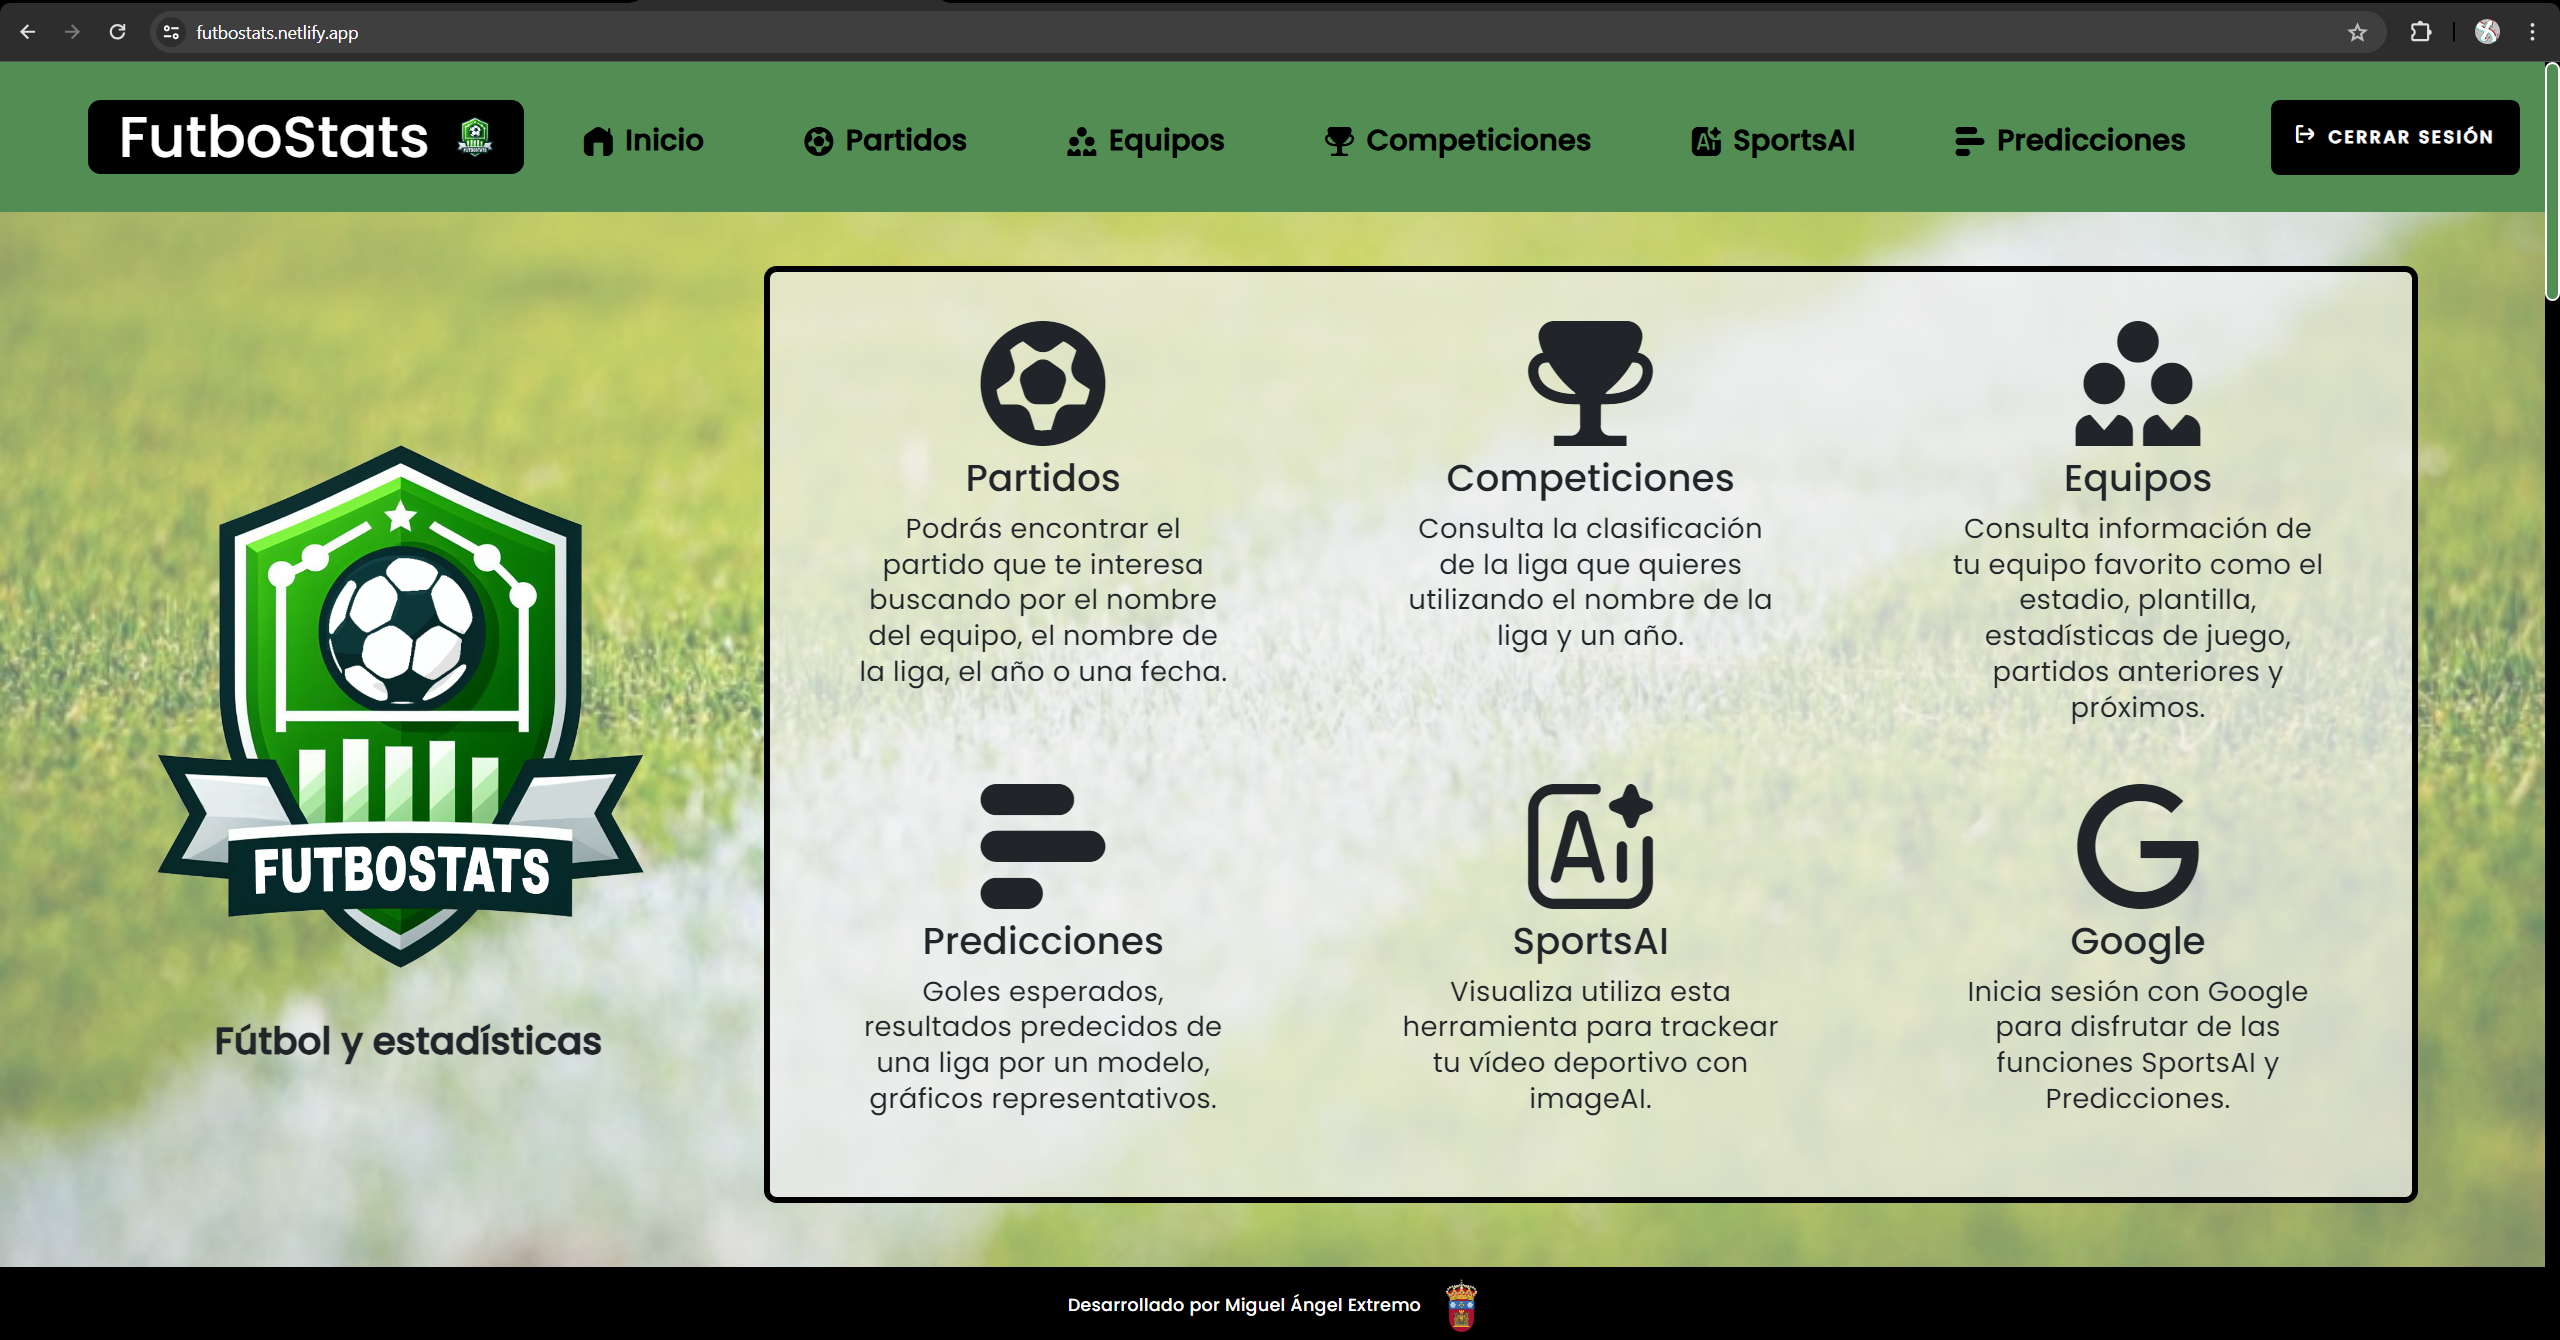
\includegraphics[width=1\linewidth]{img/inicio-UM.png}
    \caption{Inicio de FutboStats}
    \label{fig:enter-label}
\end{figure}

\begin{figure}[H]
    \centering
    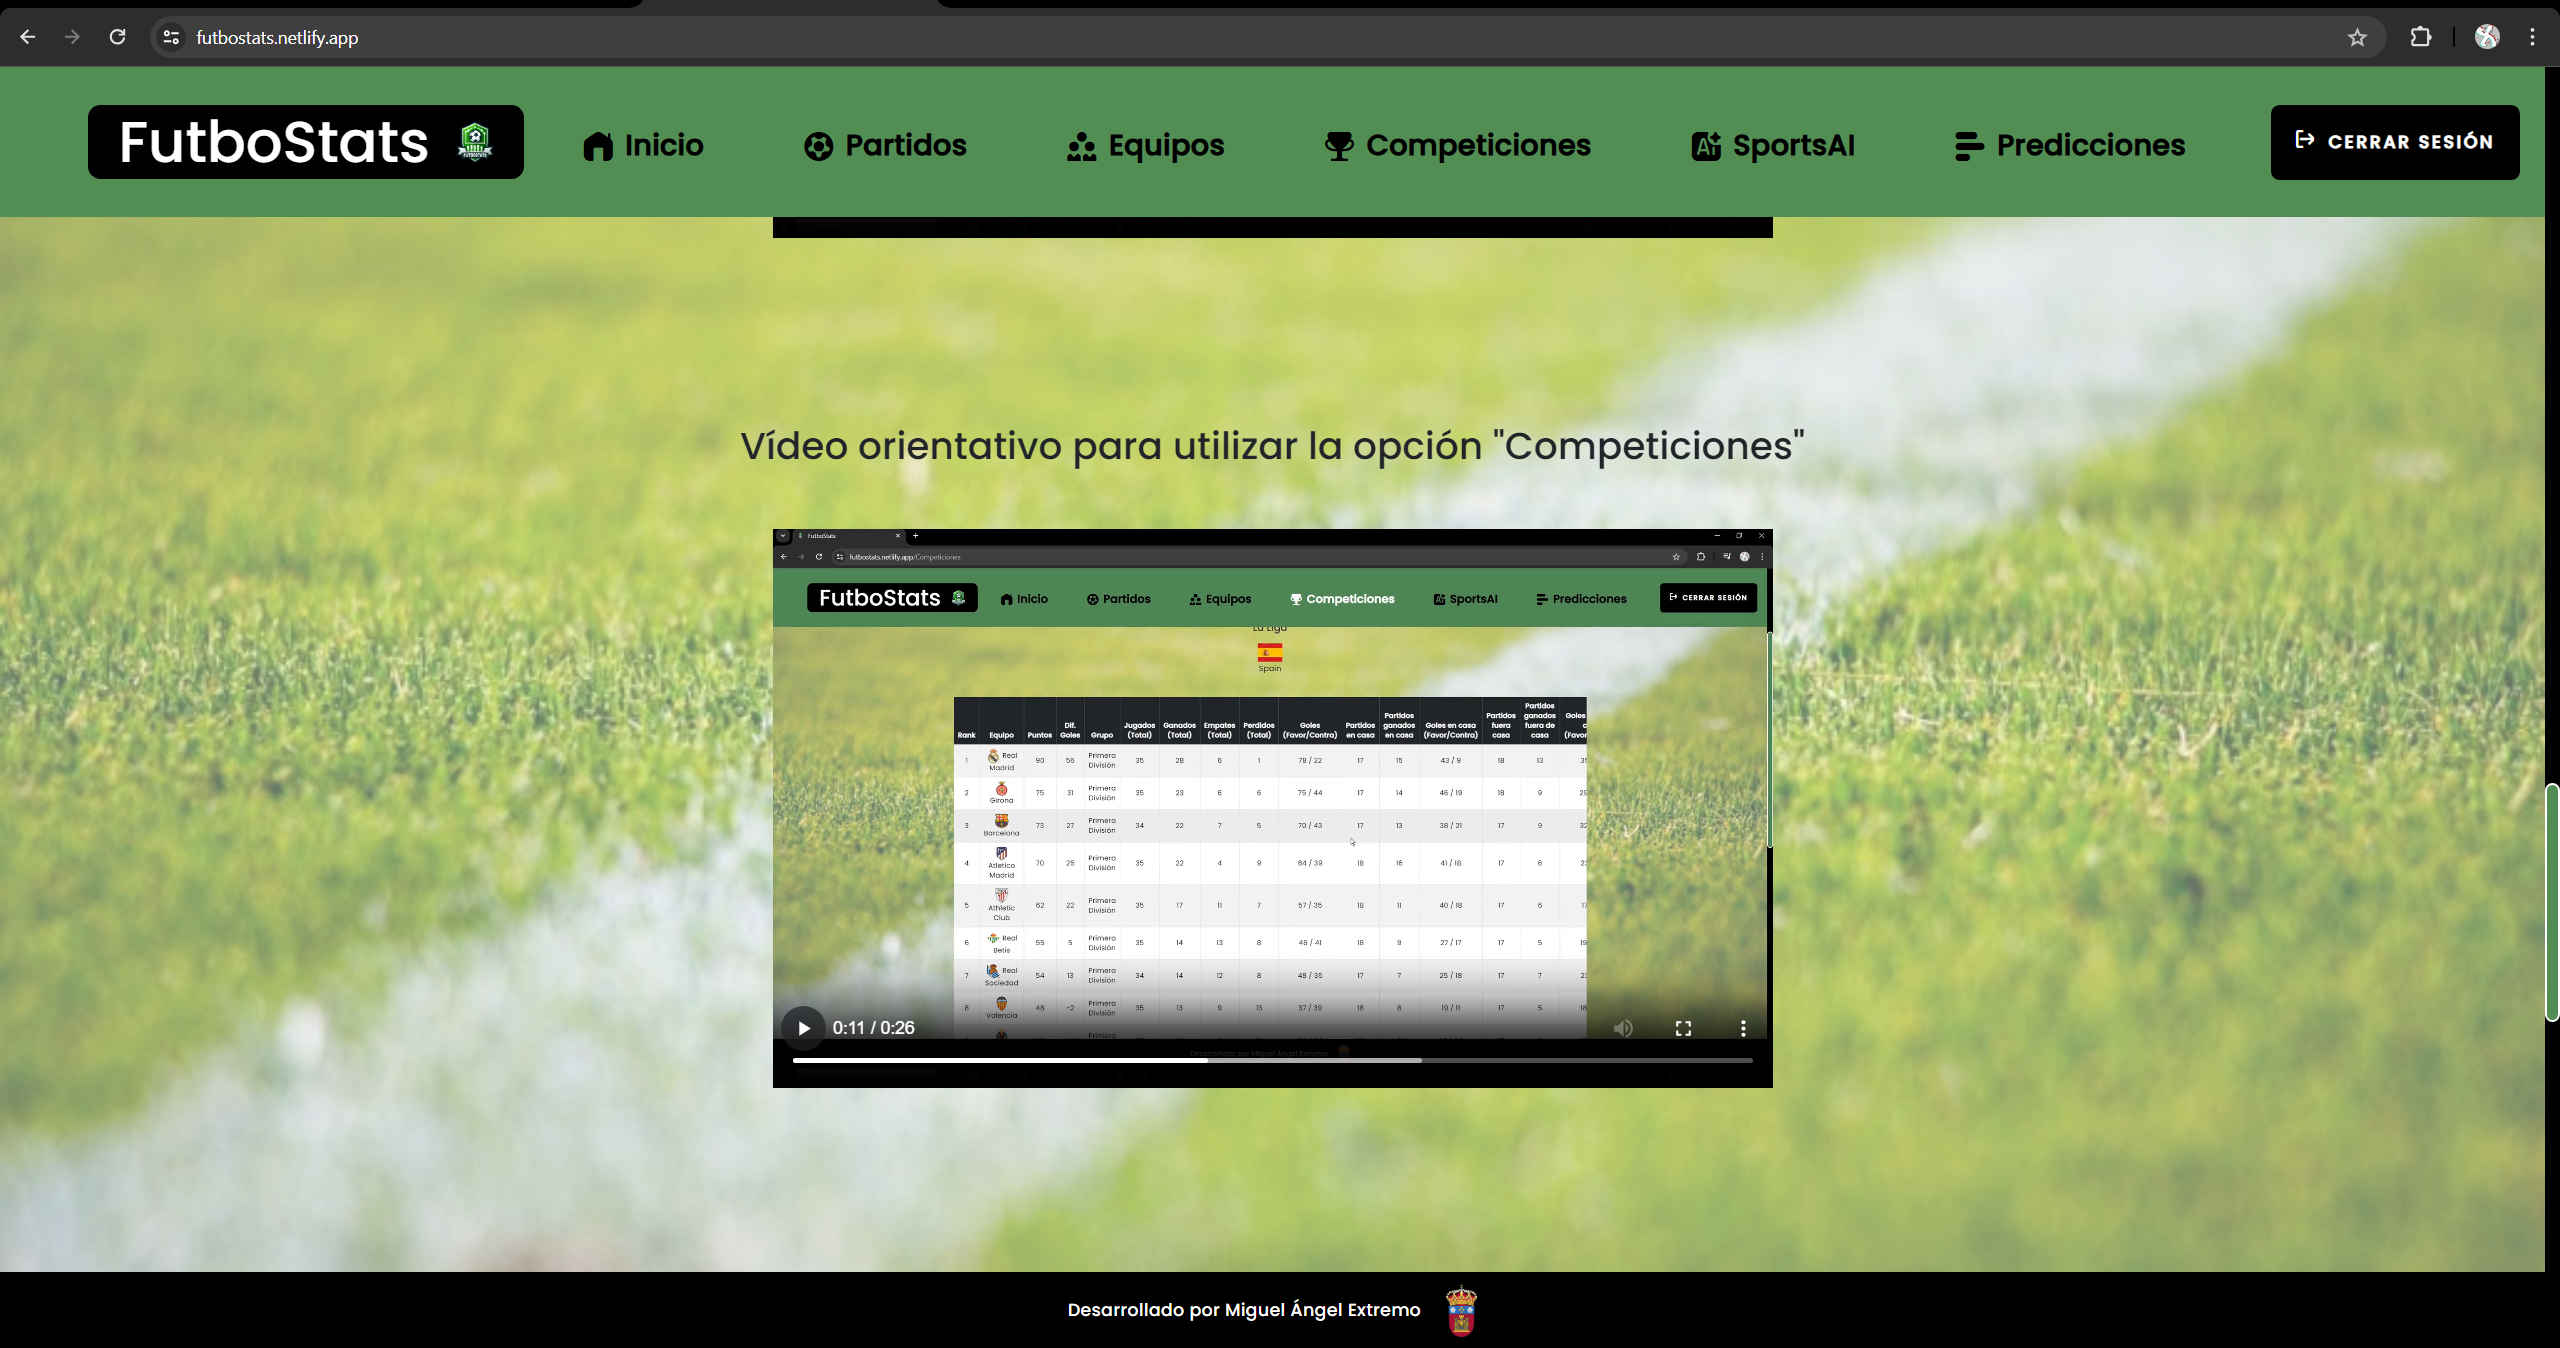
\includegraphics[width=1\linewidth]{img/inicio2-UM.png}
    \caption{Tutoriales en Inicio de FutboStats}
    \label{fig:enter-label}
\end{figure}

\subsection{Buscar partidos}
El apartado 'Partidos' de FutboStats proporciona al usuario una forma sencilla de buscar partidos introduciendo unos parámetros de búsqueda.\\
Para buscar partidos el usuario debe:
\begin{enumerate}
    \item Pulsar en el menú superior la opción 'Partidos'.
    \item Introducir el nombre de una liga. El sistema genera una lista de sugerencias al usuario a medida que este escribe.
    \item Introducir el nombre de un equipo.
    \item Introducir una fecha para filtrar los partidos.
    \item Para realizar la búsqueda de partidos es obligatorio introducir el nombre de la liga o el nombre del equipo.
    \item La fecha es un parámetro opcional para ofrecer un mayor filtrado.
    \item Por último, dar al botón buscar.
    \item El usuario visualiza los resultados de la búsqueda.
    \item En el caso de no haber partidos con esos filtros, se le informa al usuario mediante un mensaje.
\end{enumerate}

\begin{figure}[H]
    \centering
    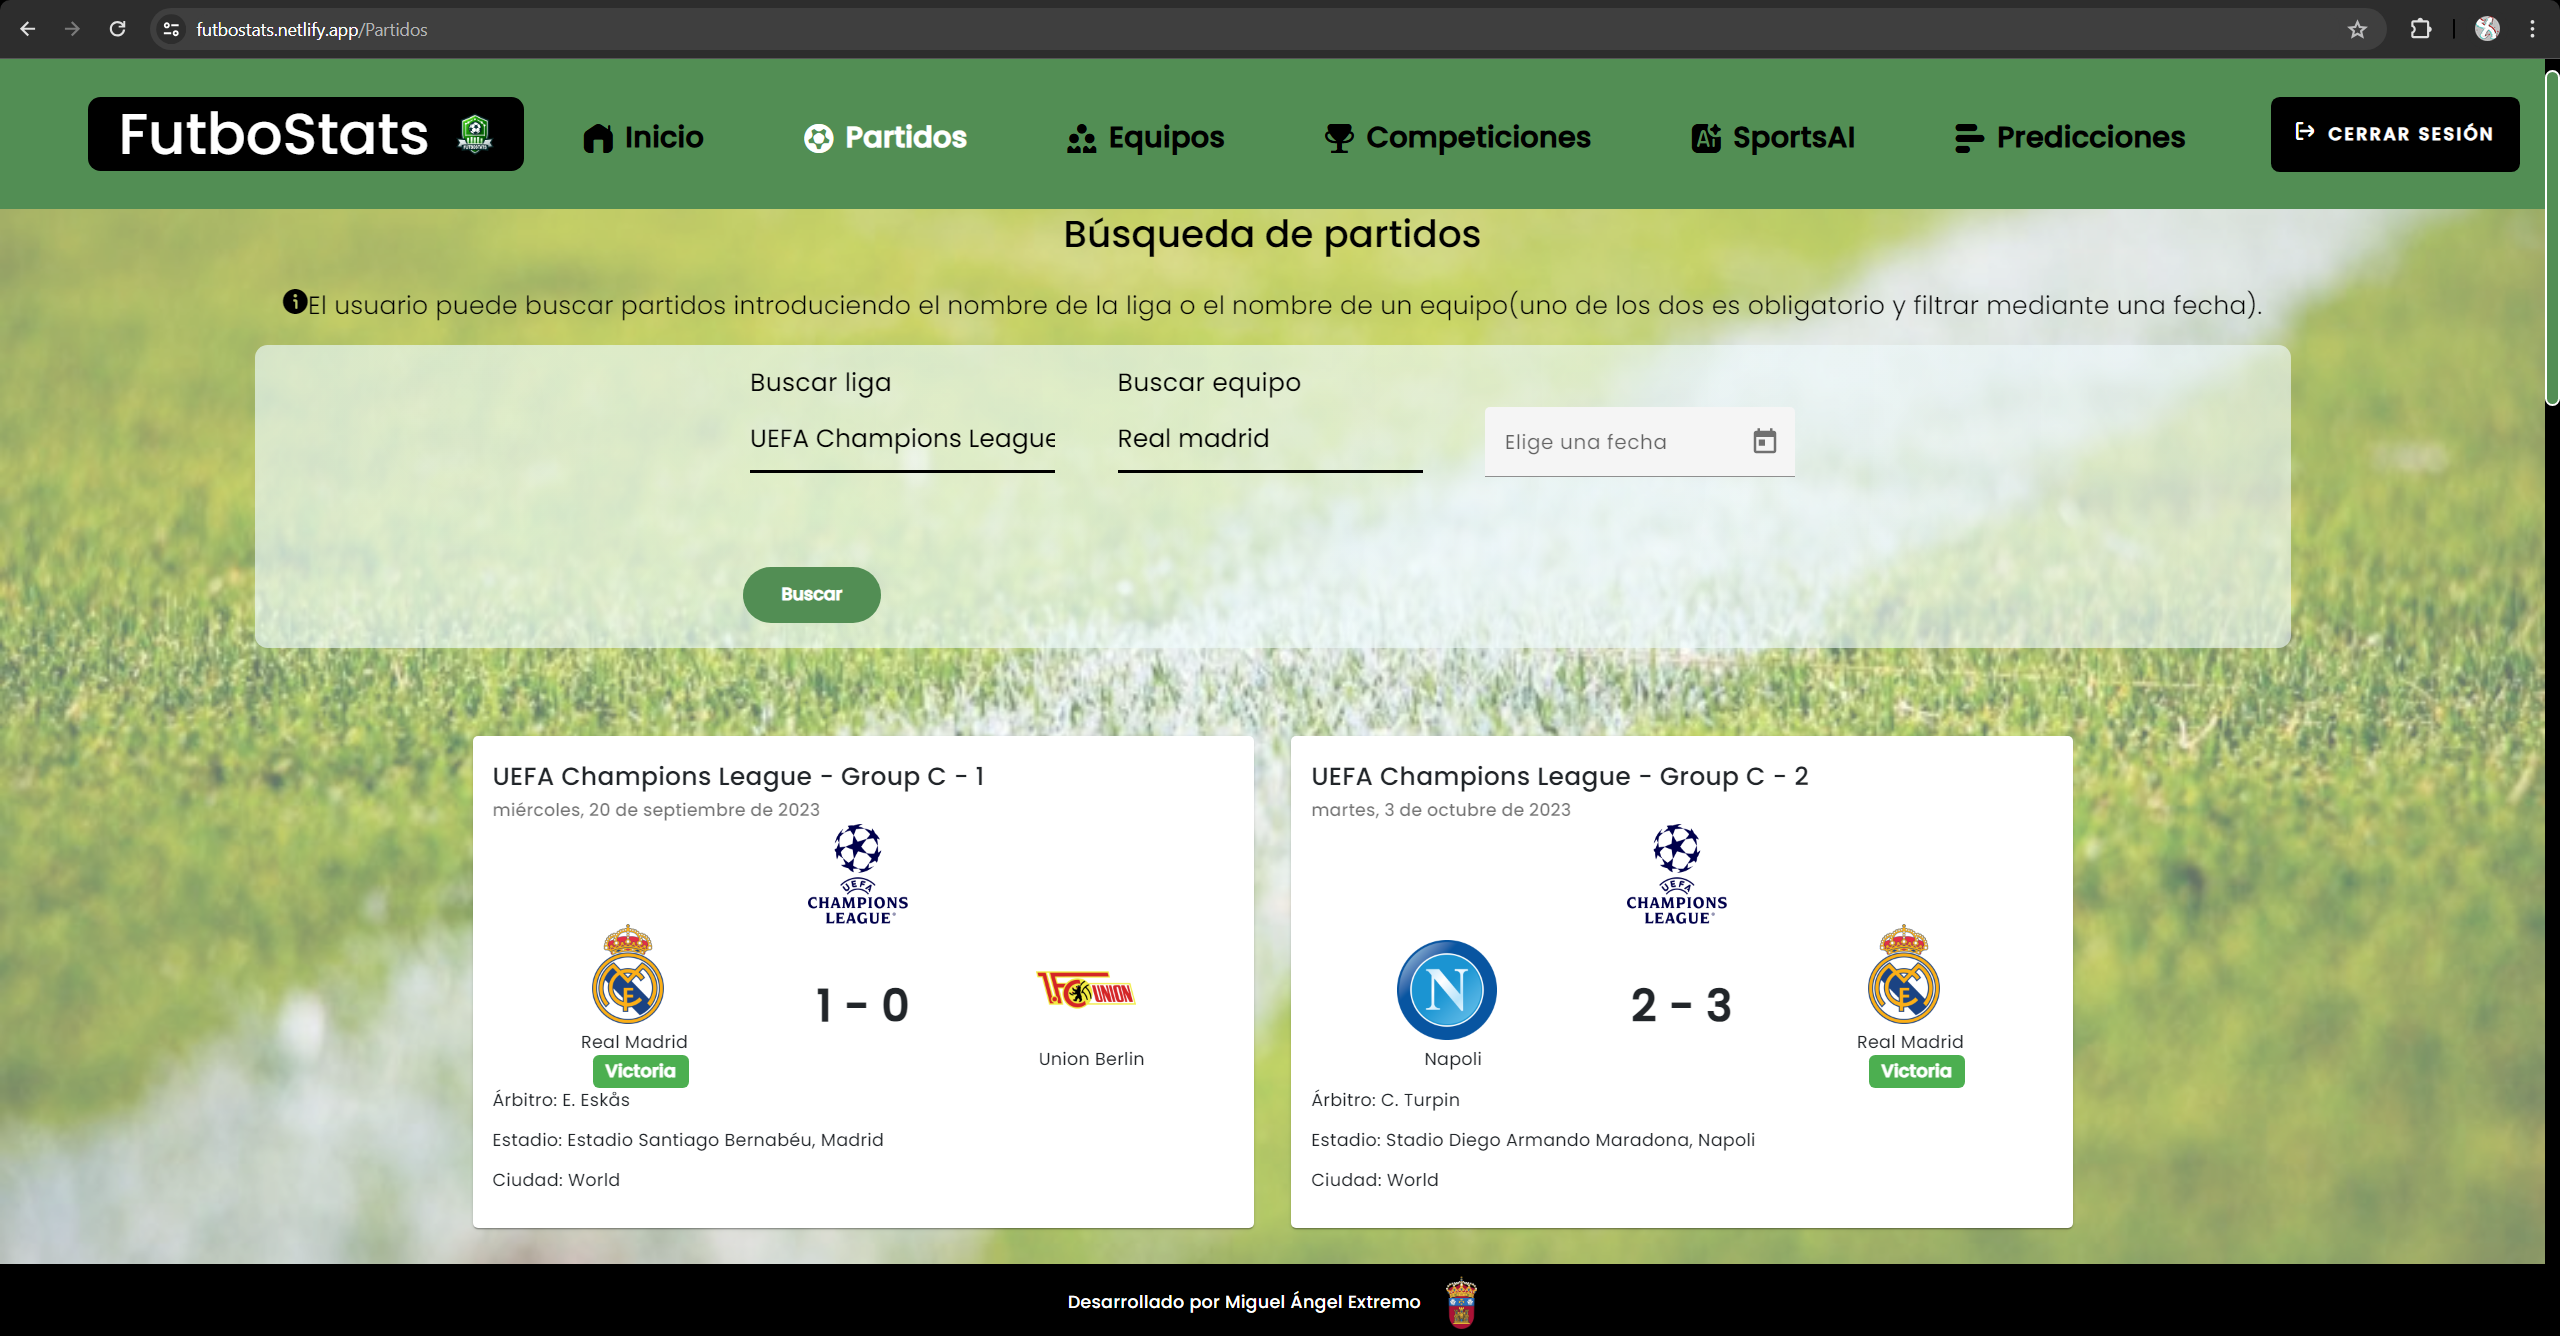
\includegraphics[width=1\linewidth]{img/partidos-UM.png}
    \caption{Búsqueda de partidos en FutboStats}
    \label{fig:enter-label}
\end{figure}

\begin{figure}[H]
    \centering
    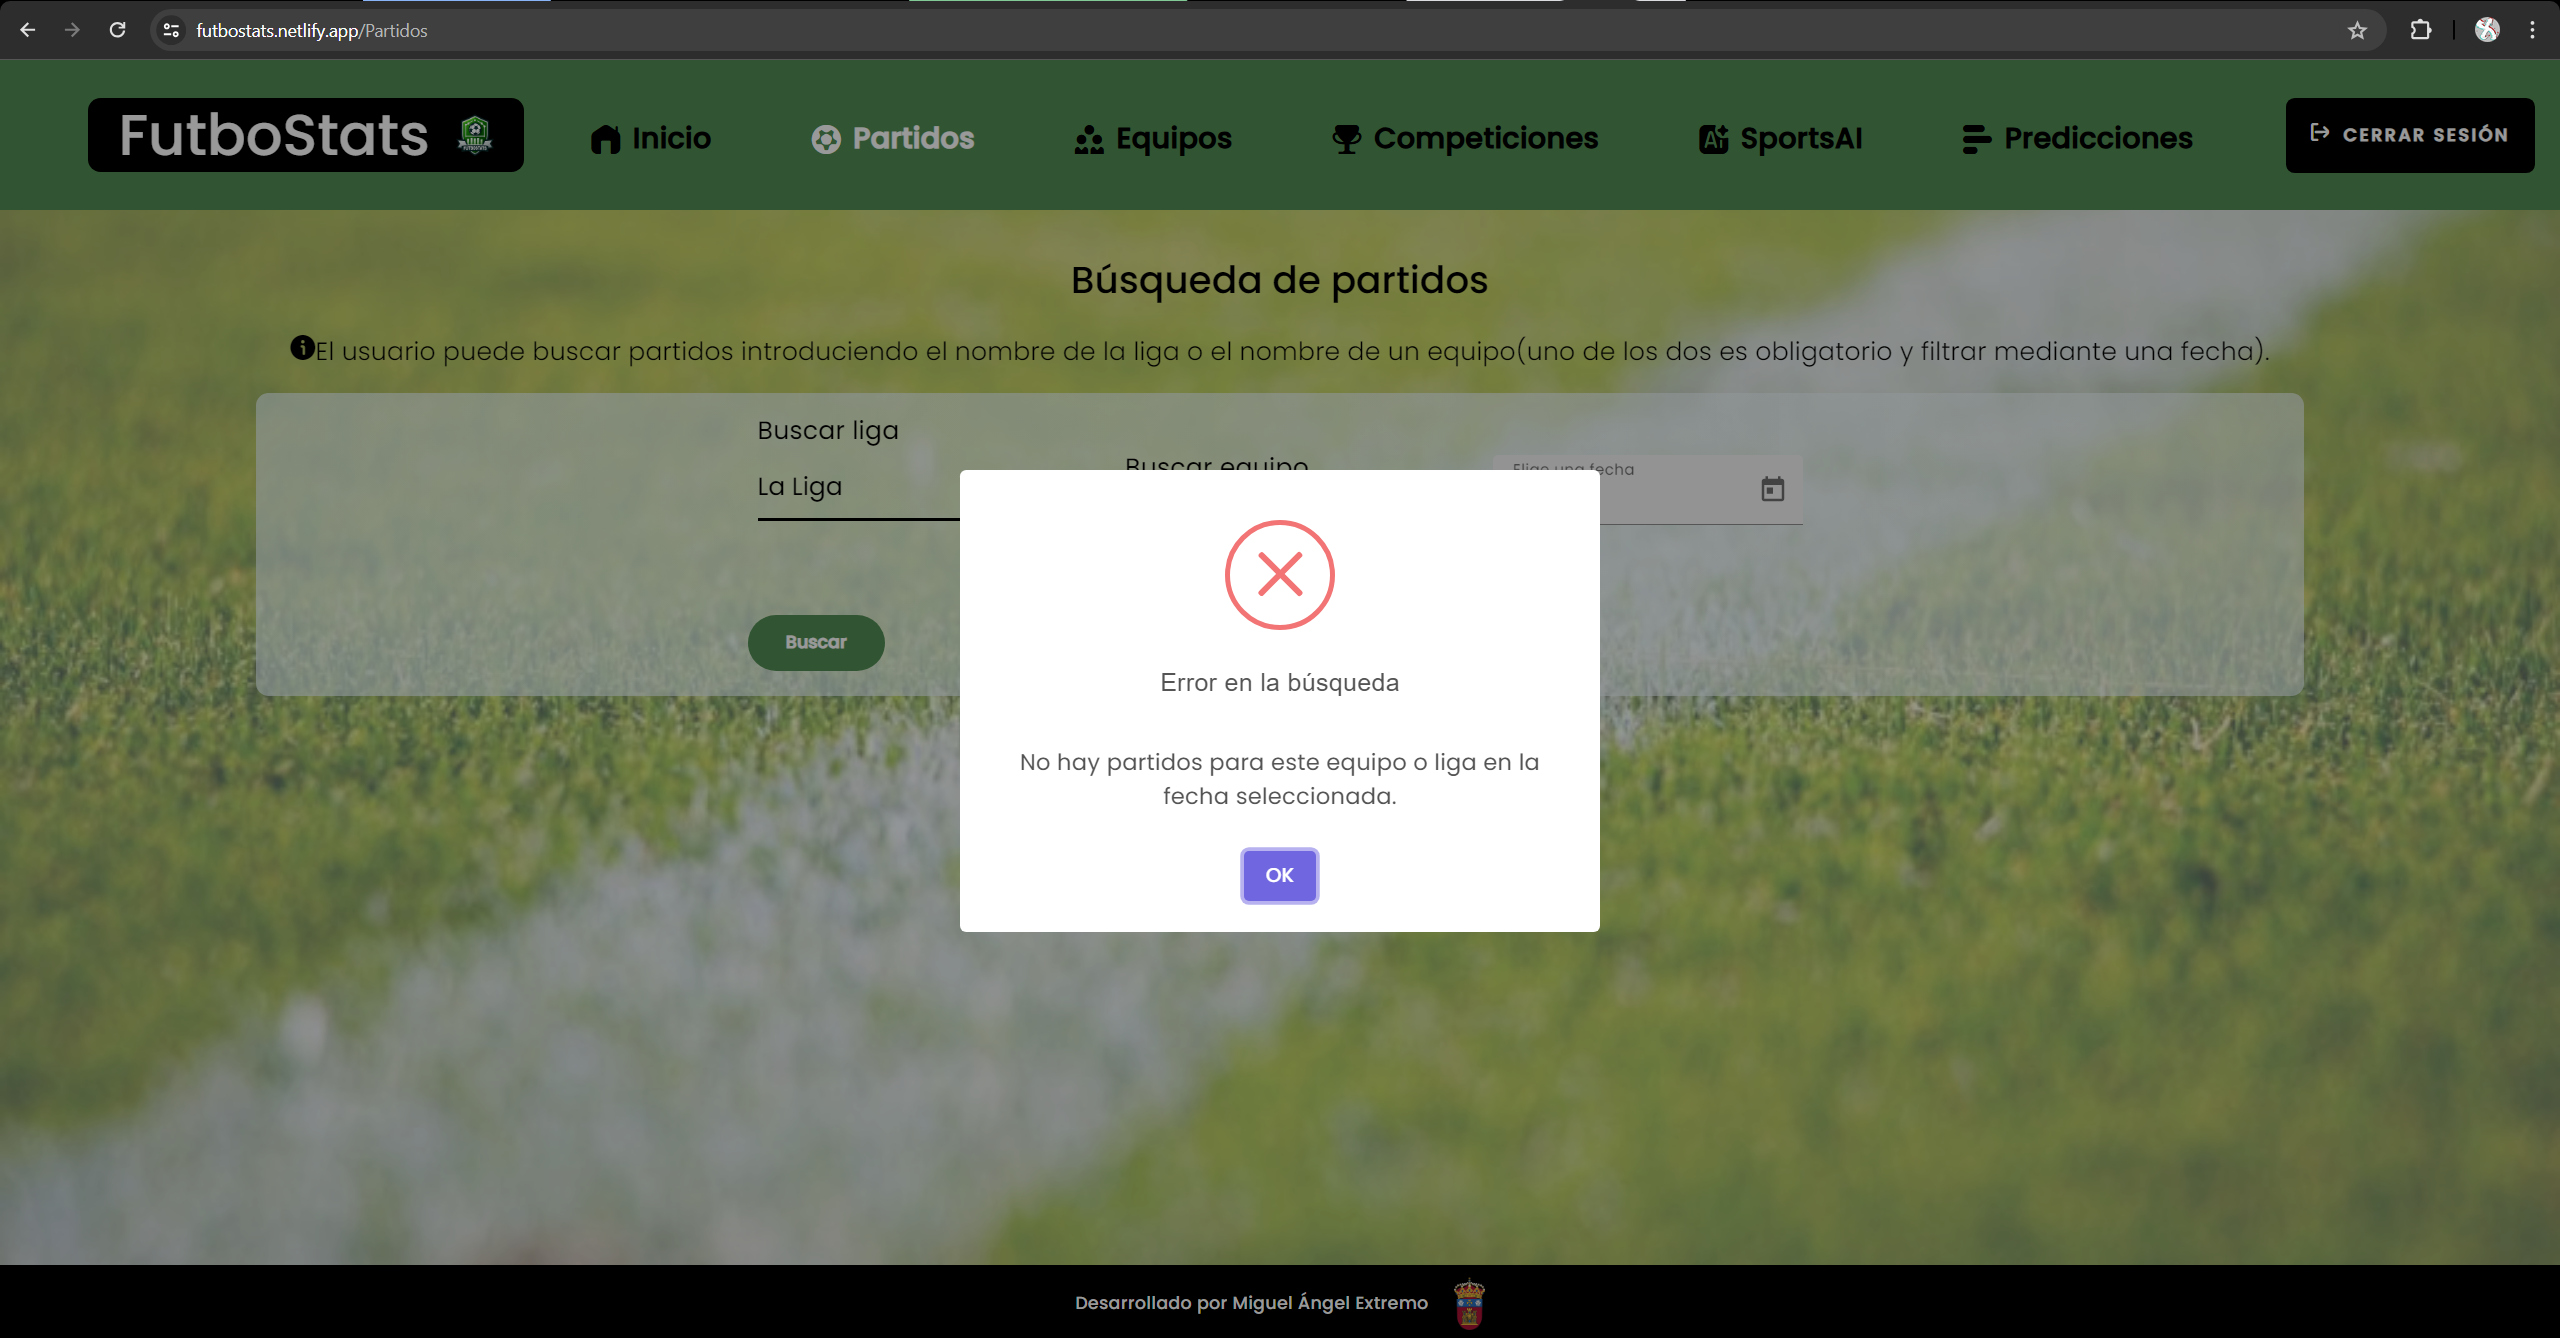
\includegraphics[width=1\linewidth]{img/partidosError-UM.png}
    \caption{Búsqueda de partidos en FutboStats sin resultados.}
    \label{fig:enter-label}
\end{figure}

\subsection{Buscar equipos}
El apartado 'Equipos' de FutboStats proporciona al usuario una forma sencilla de buscar información sobre un equipo de fútbol y consultar algunas estadísticas. \\
Para buscar equipos el usuario debe:
\begin{enumerate}
    \item Pulsar en el menú superior la opción 'Equipos'.
    \item Introducir el nombre de un equipo.
    \item Elegir un año del que quiera ver las estadísticas. Por defecto, se elige el 2023.
    \item Darle a enter o al botón de buscar para realizar la búsqueda.
    \item El usuario visualizará información del equipo como su escudo, año de fundación, estadio, liga, los cuatro partidos anteriores que ha disputado, los cuatro partidos siguientes que ha disputado, la plantilla del equipo, estadísticas sobre las tarjetas rojas y amarillas, goles a favor y en contra, alineaciones más utilizadas, estadísticas de penaltis.
\end{enumerate}

\begin{figure}[H]
    \centering
    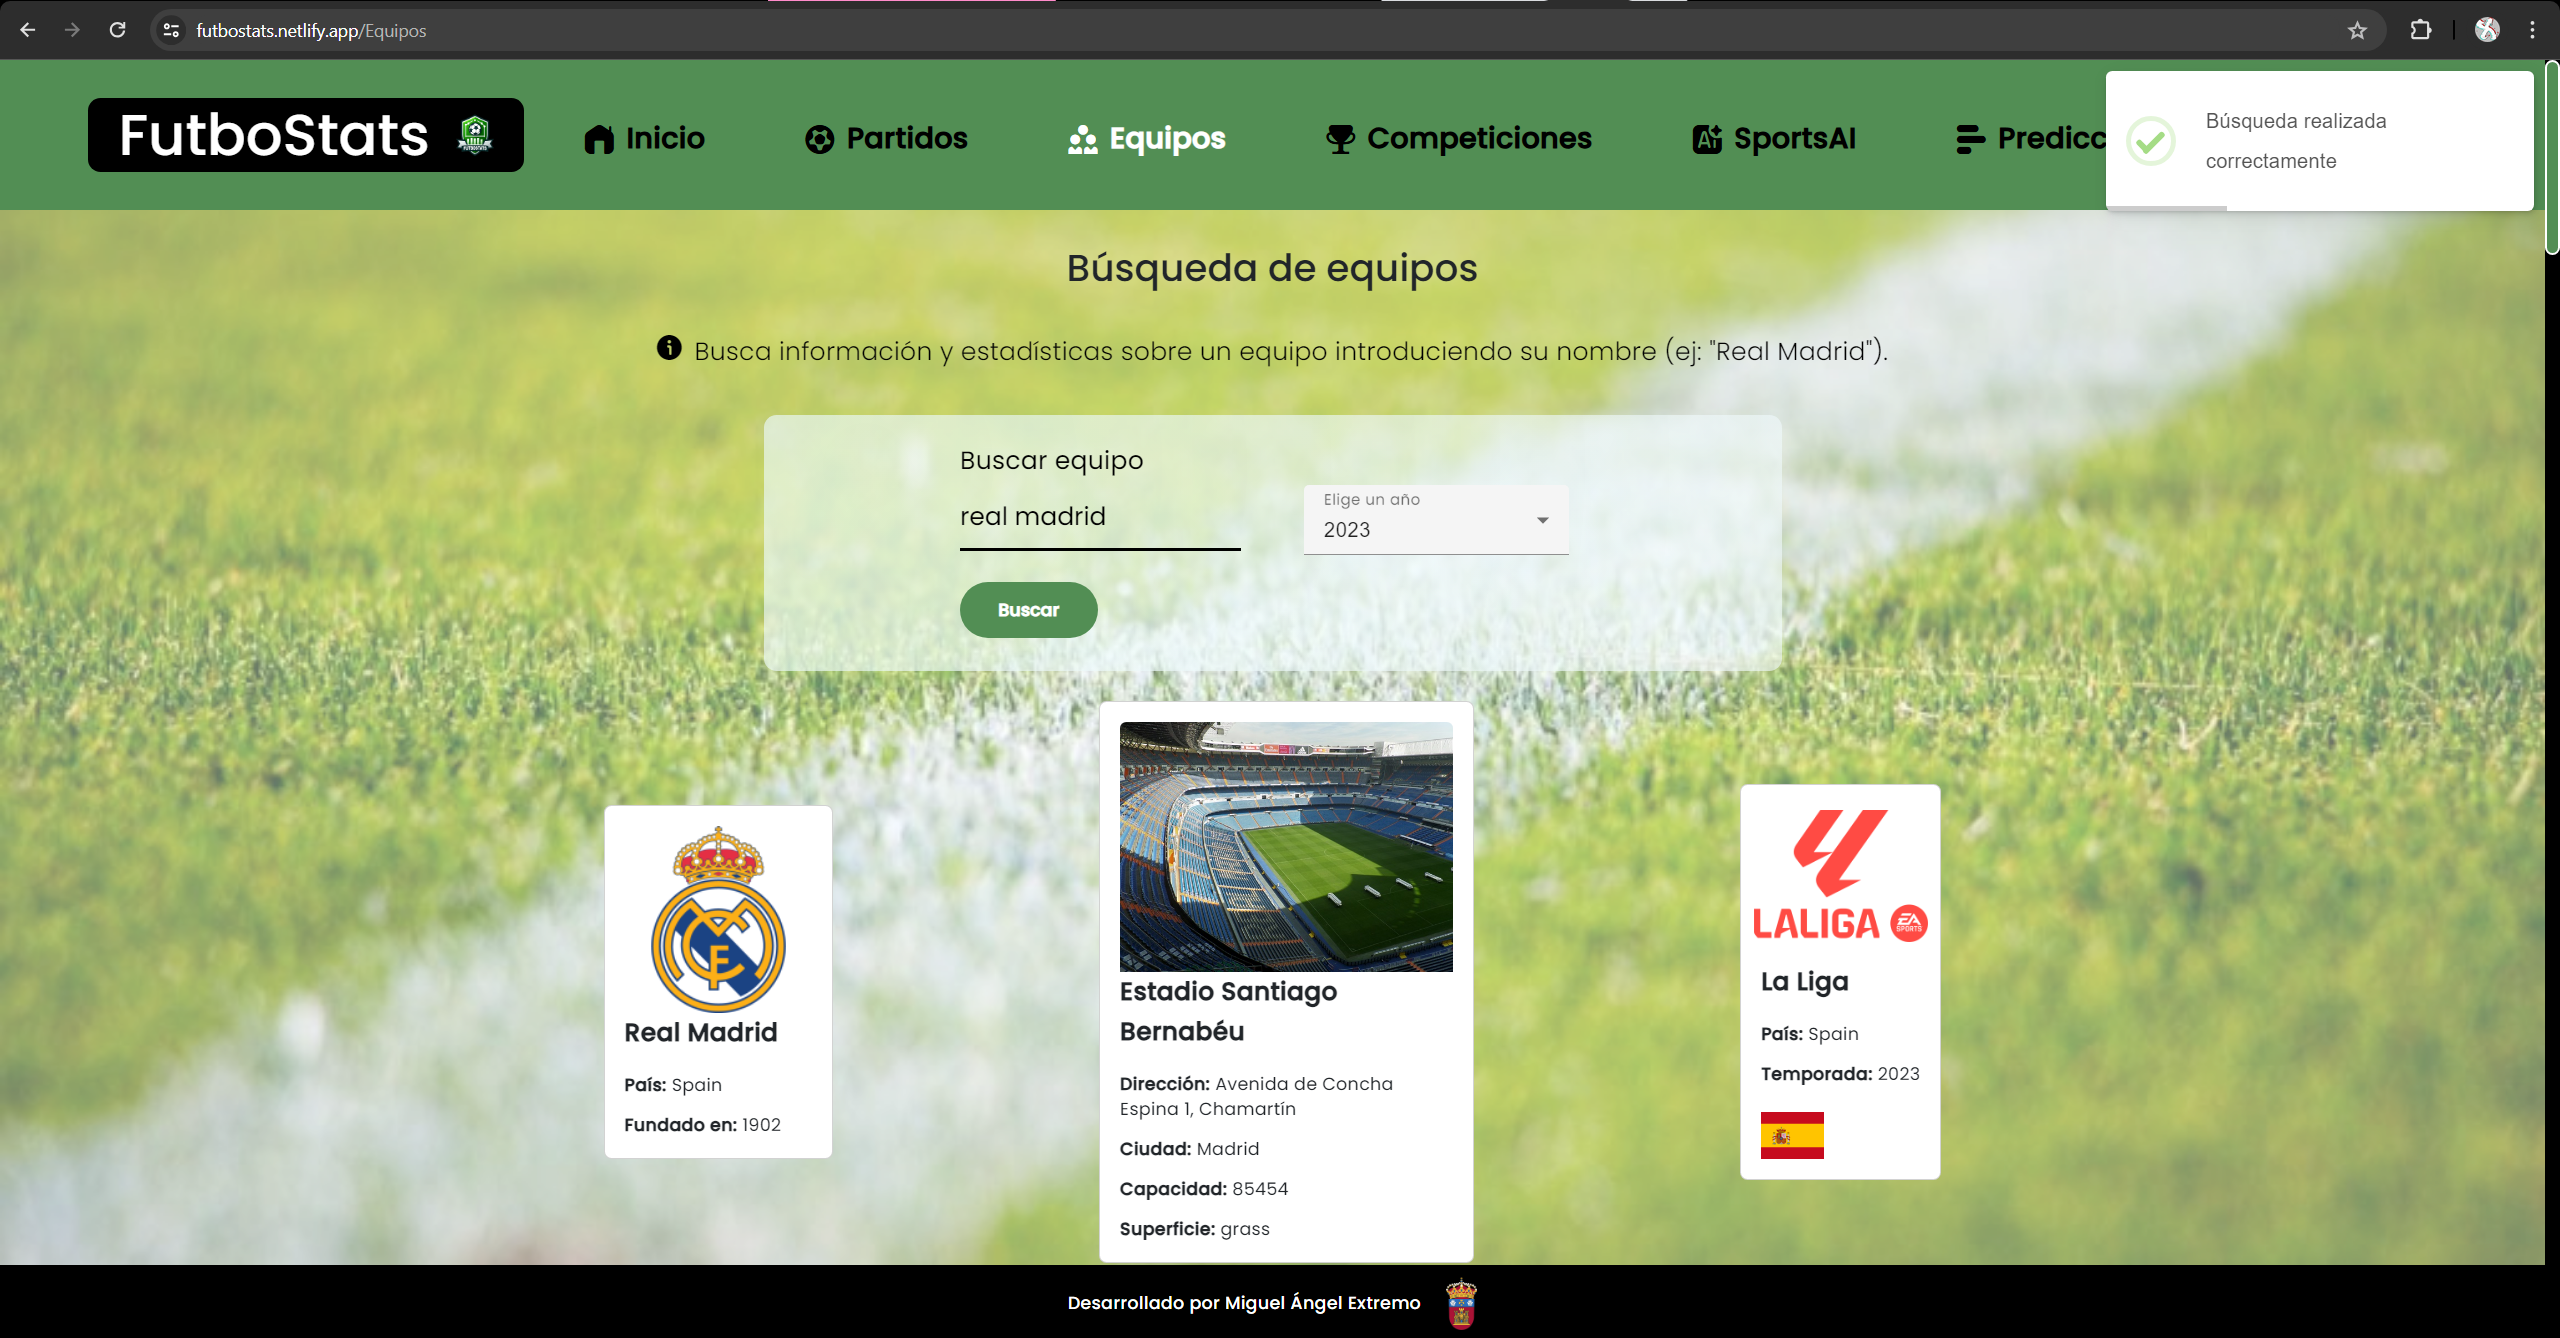
\includegraphics[width=1\linewidth]{img/busquedaEquipos.png}
    \caption{Búsqueda de equipos en FutboStats.}
    \label{fig:enter-label}
\end{figure}



\subsection{Buscar clasificaciones}
El apartado 'Competiciones' de FutboStats permite al usuario consultar la clasificación de una liga de forma sencilla. \\
Para buscar clasificaciones el usuario debe:
\begin{enumerate}
    \item Pulsar en el menú superior la opción 'Competiciones'.
    \item Introducir el nombre de la competición. El sistema genera una lista de sugerencias al usuario a medida que este escribe.
    \item Pulsar en una de las sugerencias y dar al botón de buscar.
    \item Elegir el año del que se quiere ver la clasificación. Por defecto se elige el 2023.
    \item El usuario visualizará una tabla que muestra la clasificación de la liga seleccionada.
    \item Si se cambia el año, la tabla cambiará para mostrar la información del nuevo año seleccionado.
\end{enumerate}

\begin{figure}[H]
    \centering
    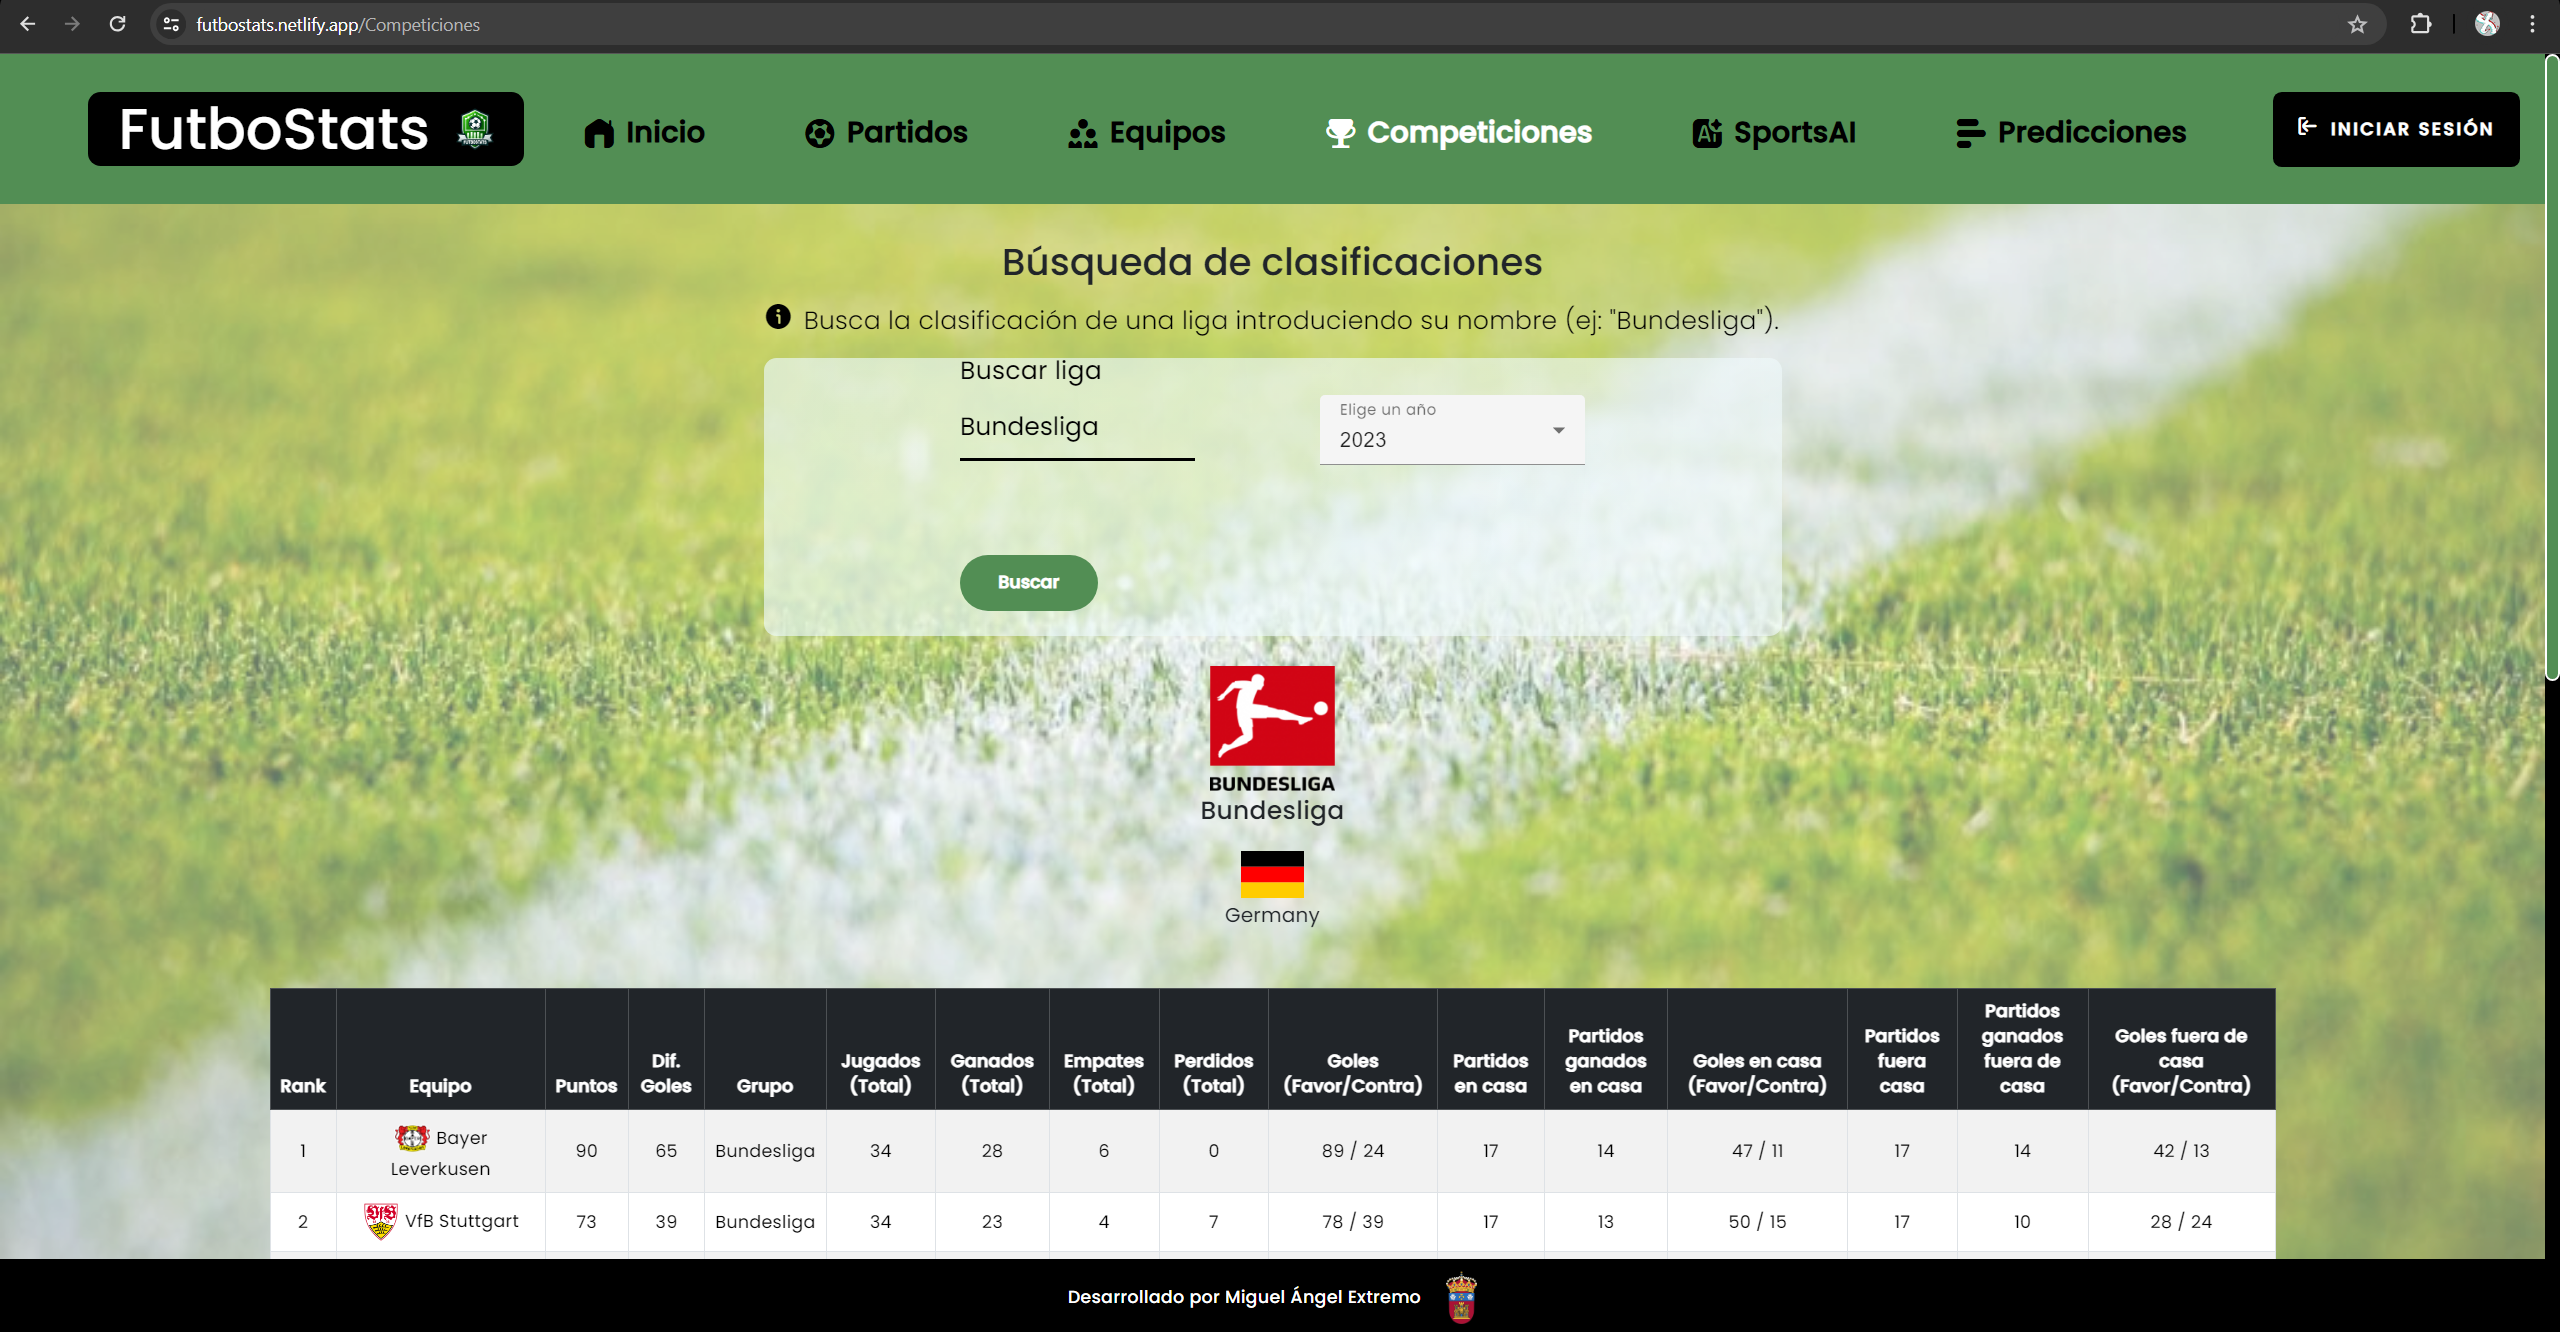
\includegraphics[width=1\linewidth]{img/buscarCompeticiones.png}
    \caption{Búsqueda de competiciones en FutboStats.}
    \label{fig:enter-label}
\end{figure}

\subsection{Iniciar sesión en FutboStats}
Si el usuario quiere utilizar las opciones 'SportsAI' y 'Predicciones' deberá iniciar sesión en la aplicación. La forma de iniciar sesión es muy sencilla, para ello el usuario deberá:
\begin{enumerate}
    \item Pulsar en el botón de iniciar sesión o en las opciones 'SportsAI' o 'Predicciones', las cuáles al no estar autenticado redirigen al usuario a la pantalla de inicio de sesión.
    \item En la pantalla de iniciar sesión, pulsar de nuevo en el botón 'Iniciar sesión' dentro del recuadro debajo del logotipo de Google.
    \item Se redirige al usuario para que se registre con su cuenta de Google.
    \item Una vez registrado, se redirige al usuario de nuevo a la página de 'Inicio' de FutboStats.
    \item El usuario puede acceder a las funcionalidades protegidas de la aplicación.
\end{enumerate}

\begin{figure}[H]
    \centering
    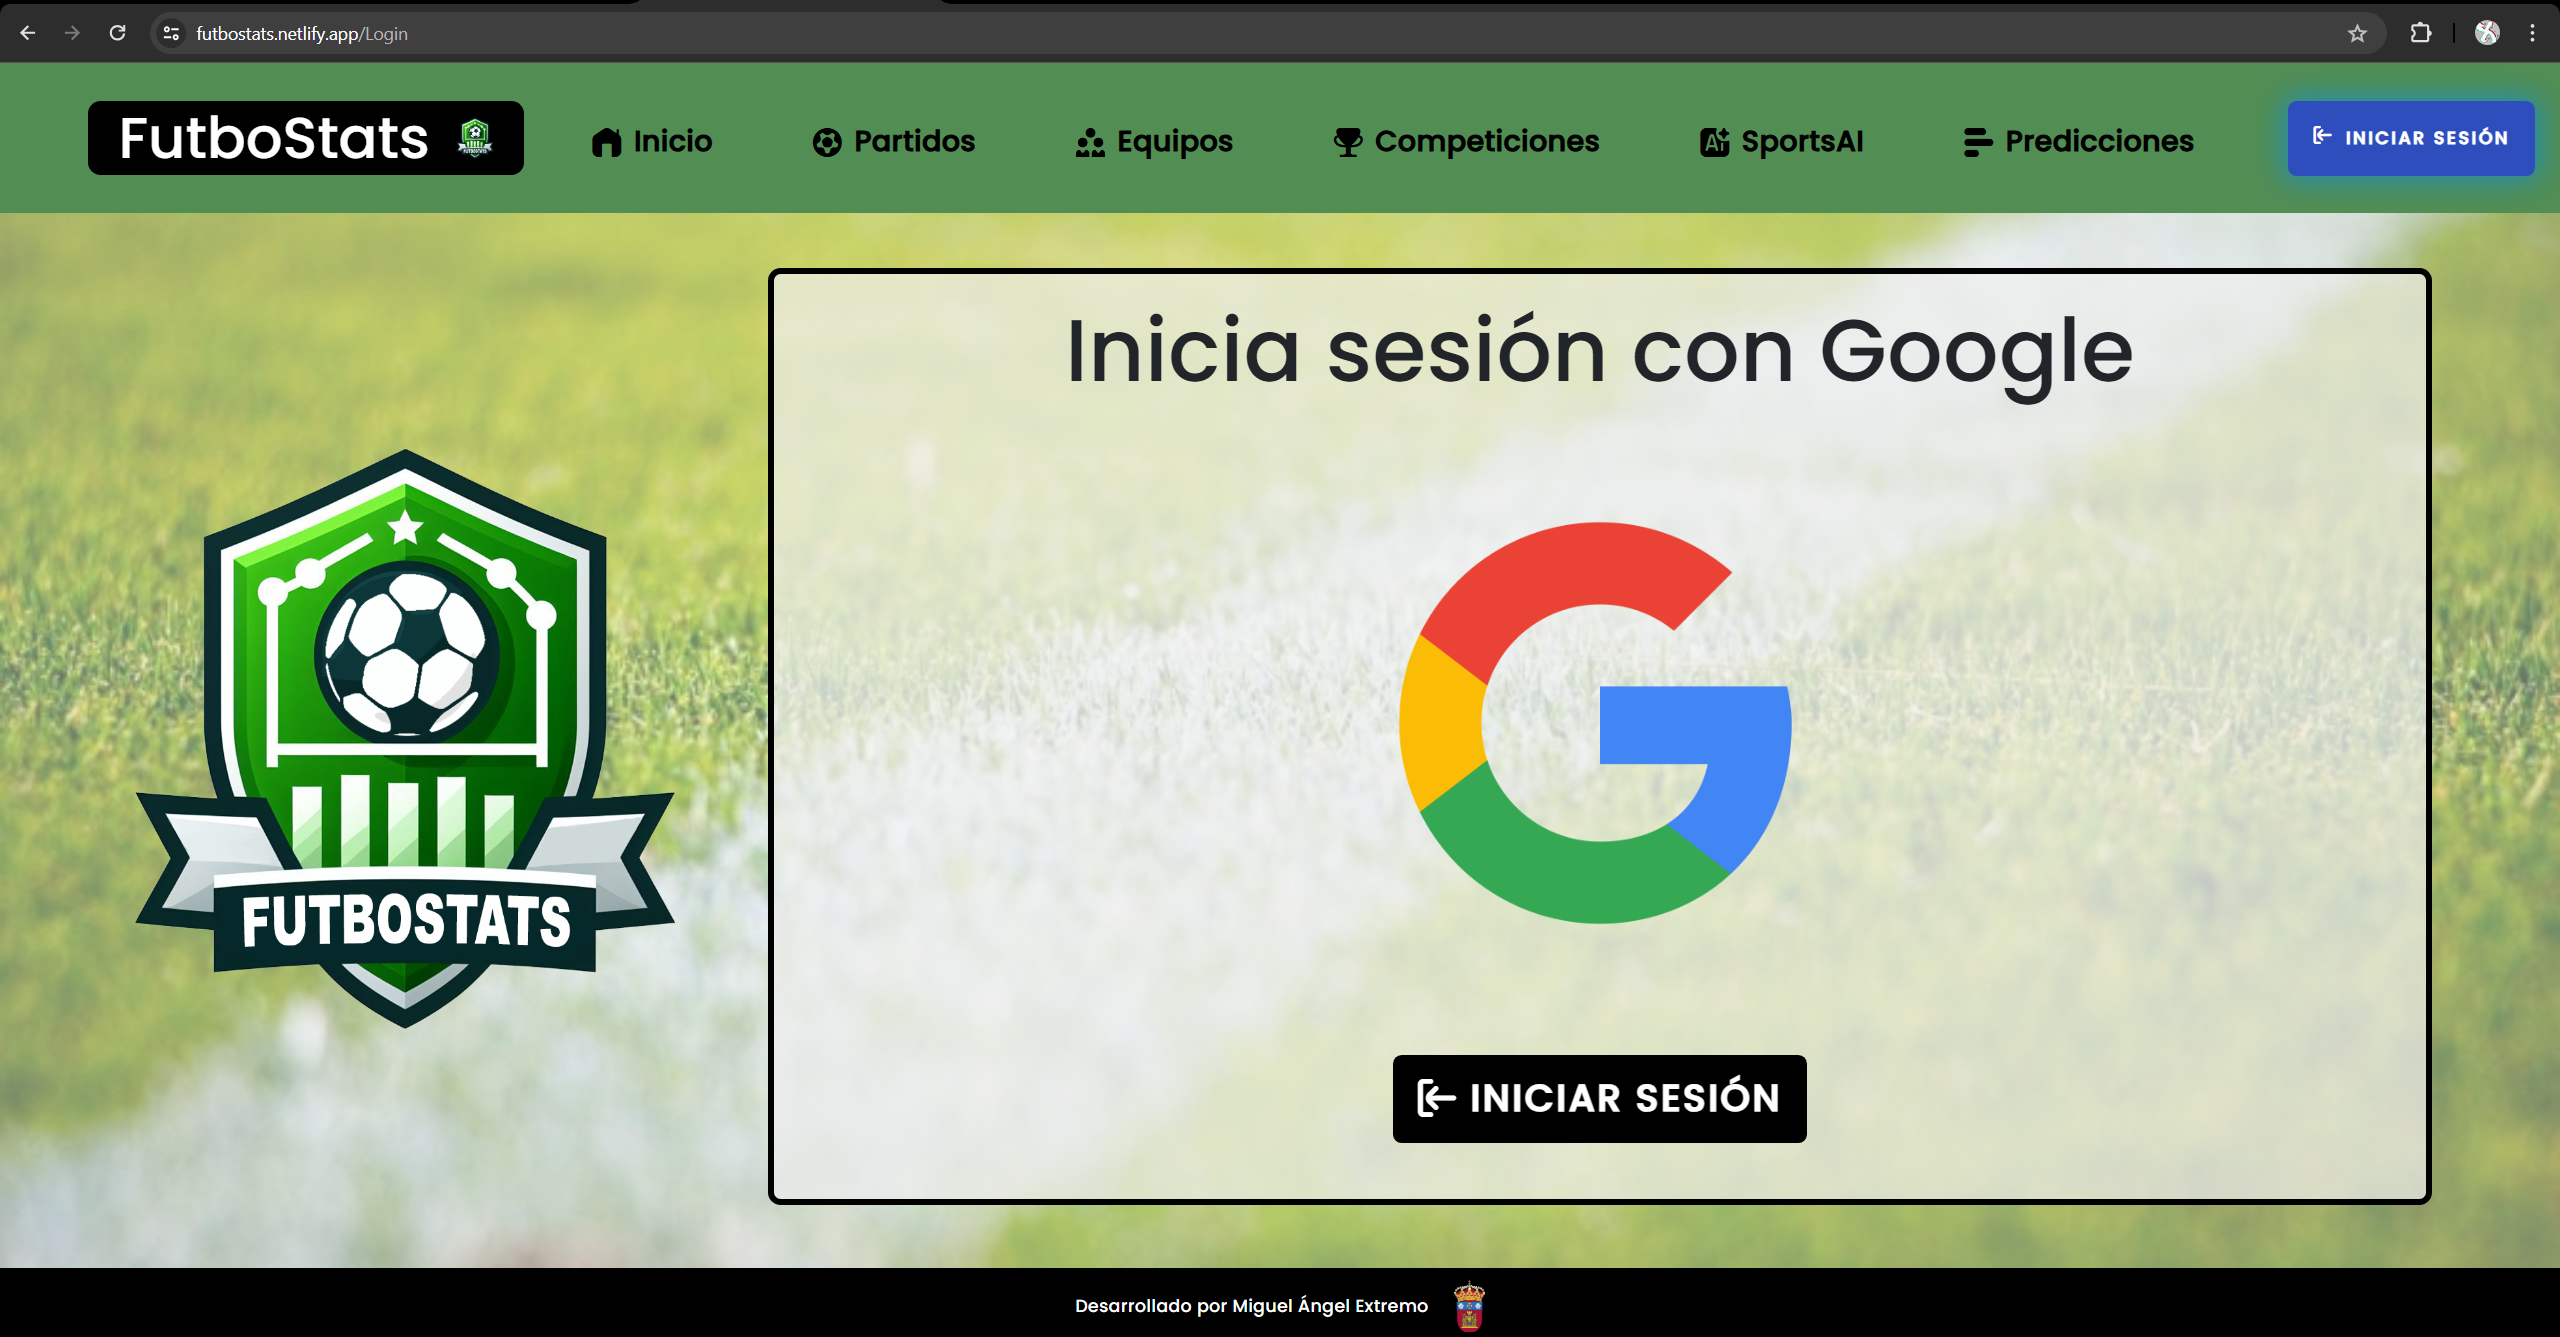
\includegraphics[width=1\linewidth]{img/iniciarSesion-UM.png}
    \caption{Paso 1 de iniciar sesión en FutboStats: entrar en iniciar sesión.}
    \label{fig:enter-label}
\end{figure}

\begin{figure}[H]
    \centering
    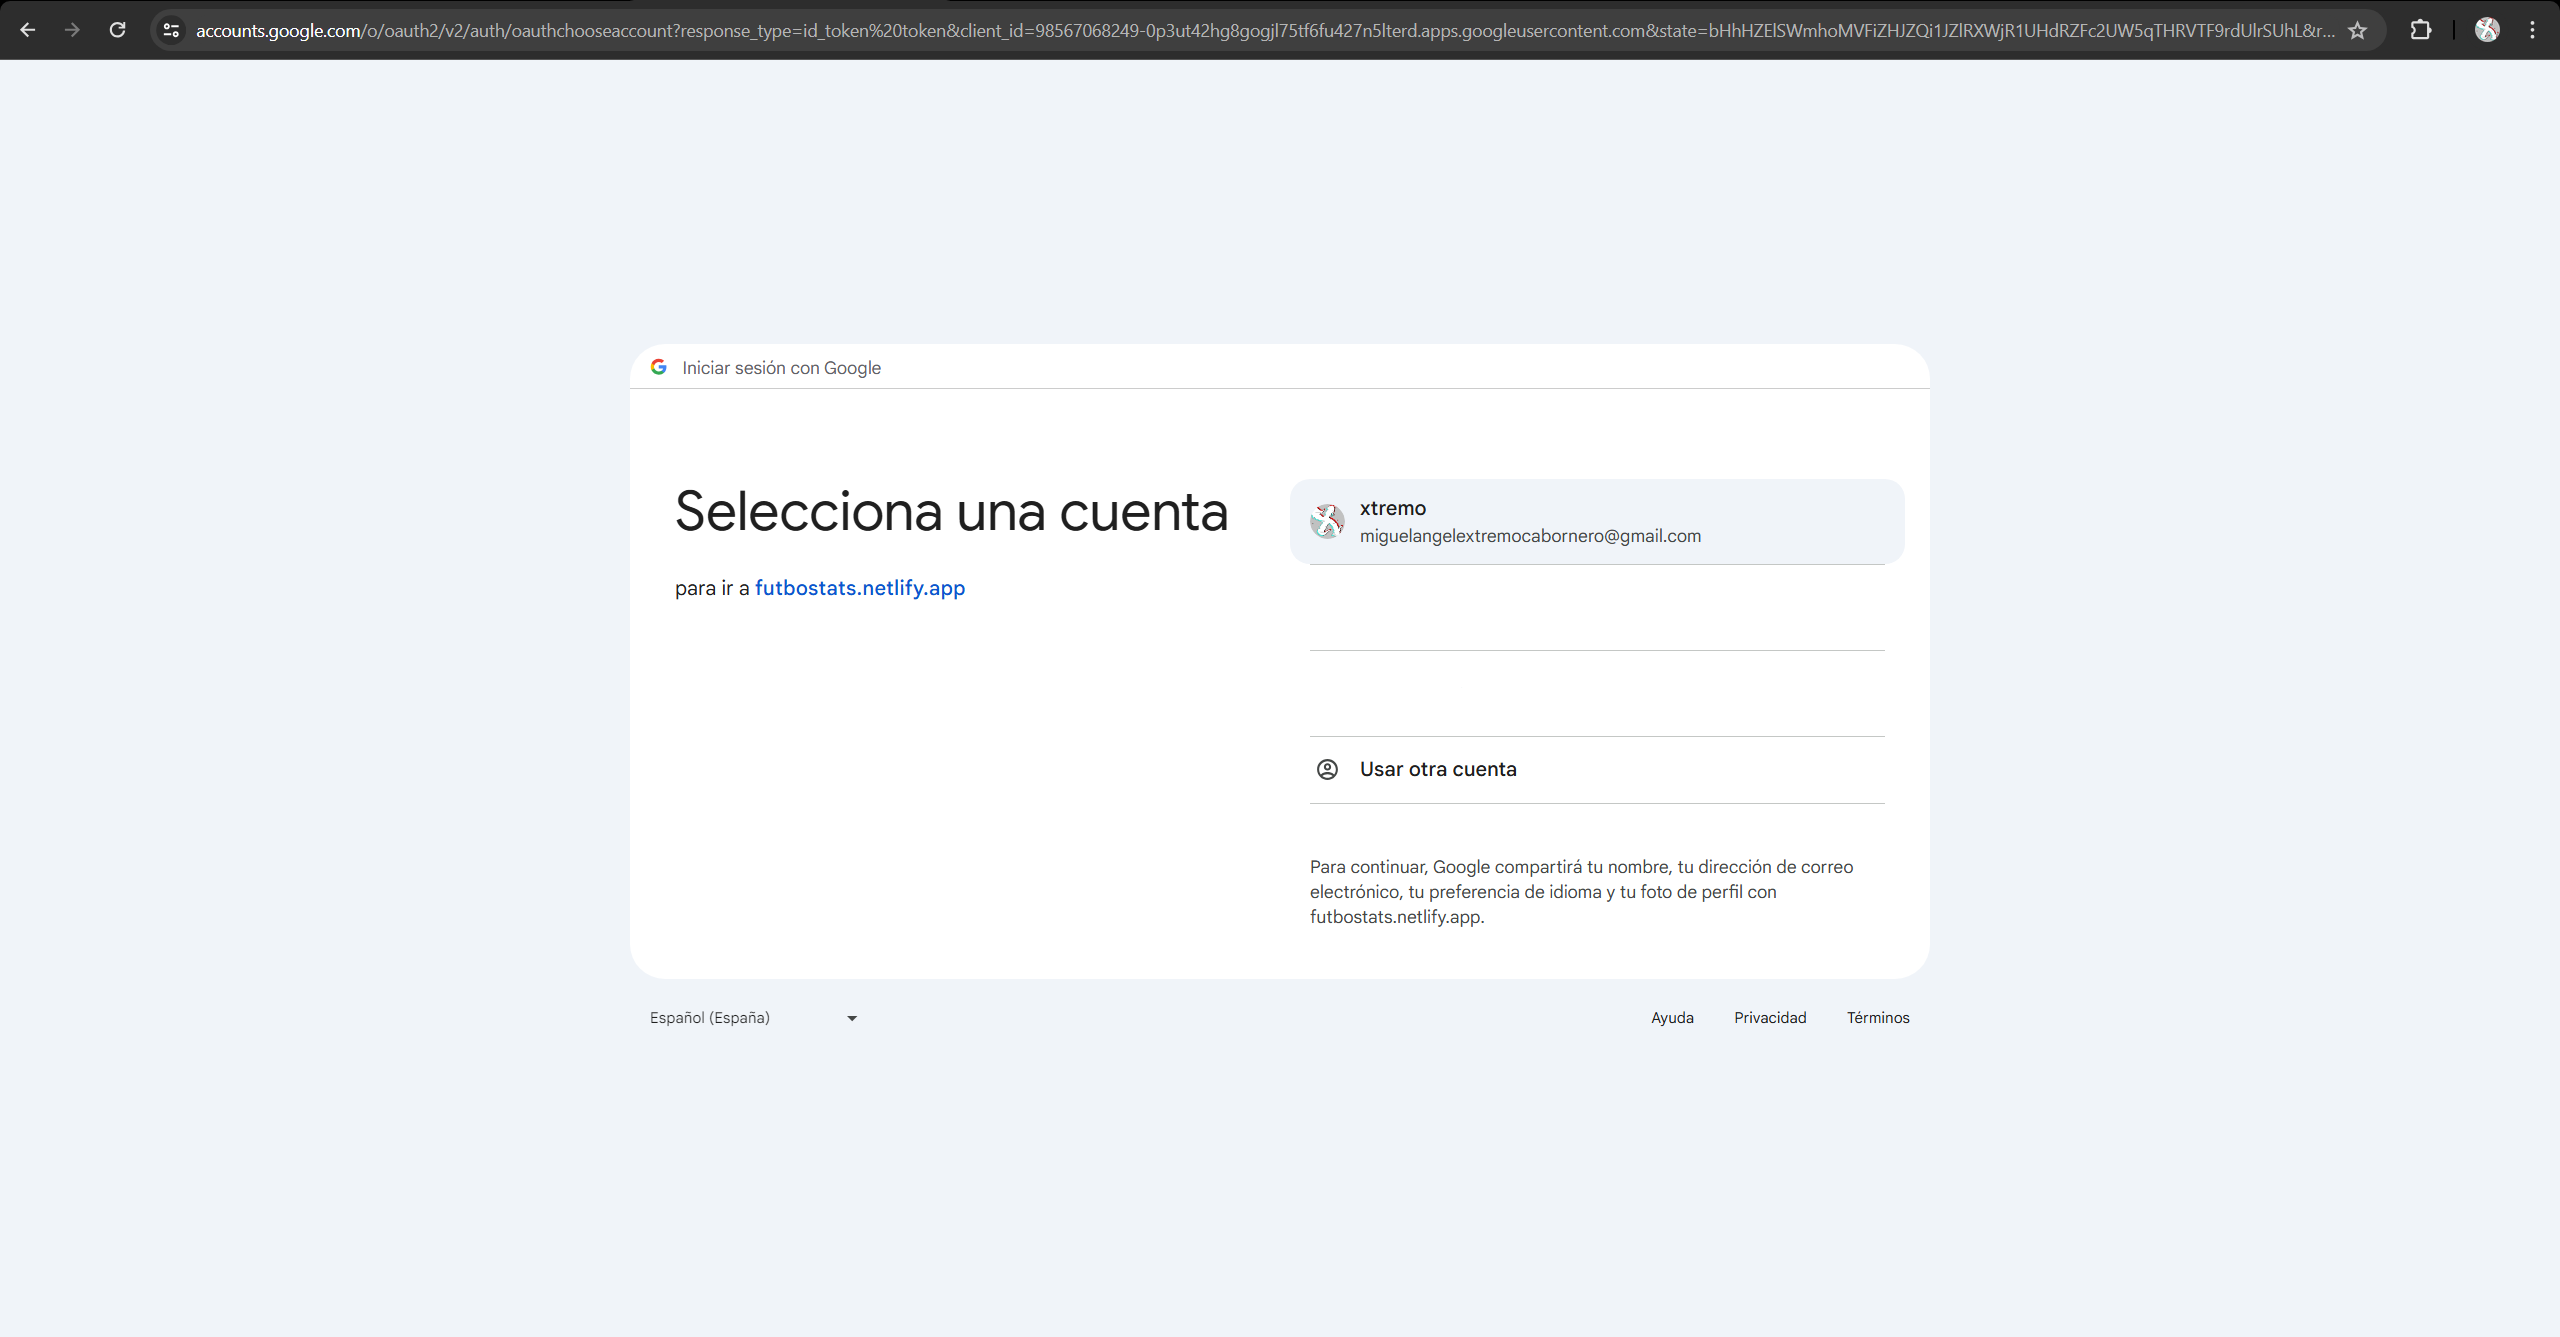
\includegraphics[width=1\linewidth]{img/iniciarSesion2-UM.png}
    \caption{Paso 2 de iniciar sesión en FutboStats: elegir la cuenta de Google.}
    \label{fig:enter-label}
\end{figure}

\begin{figure}[H]
    \centering
    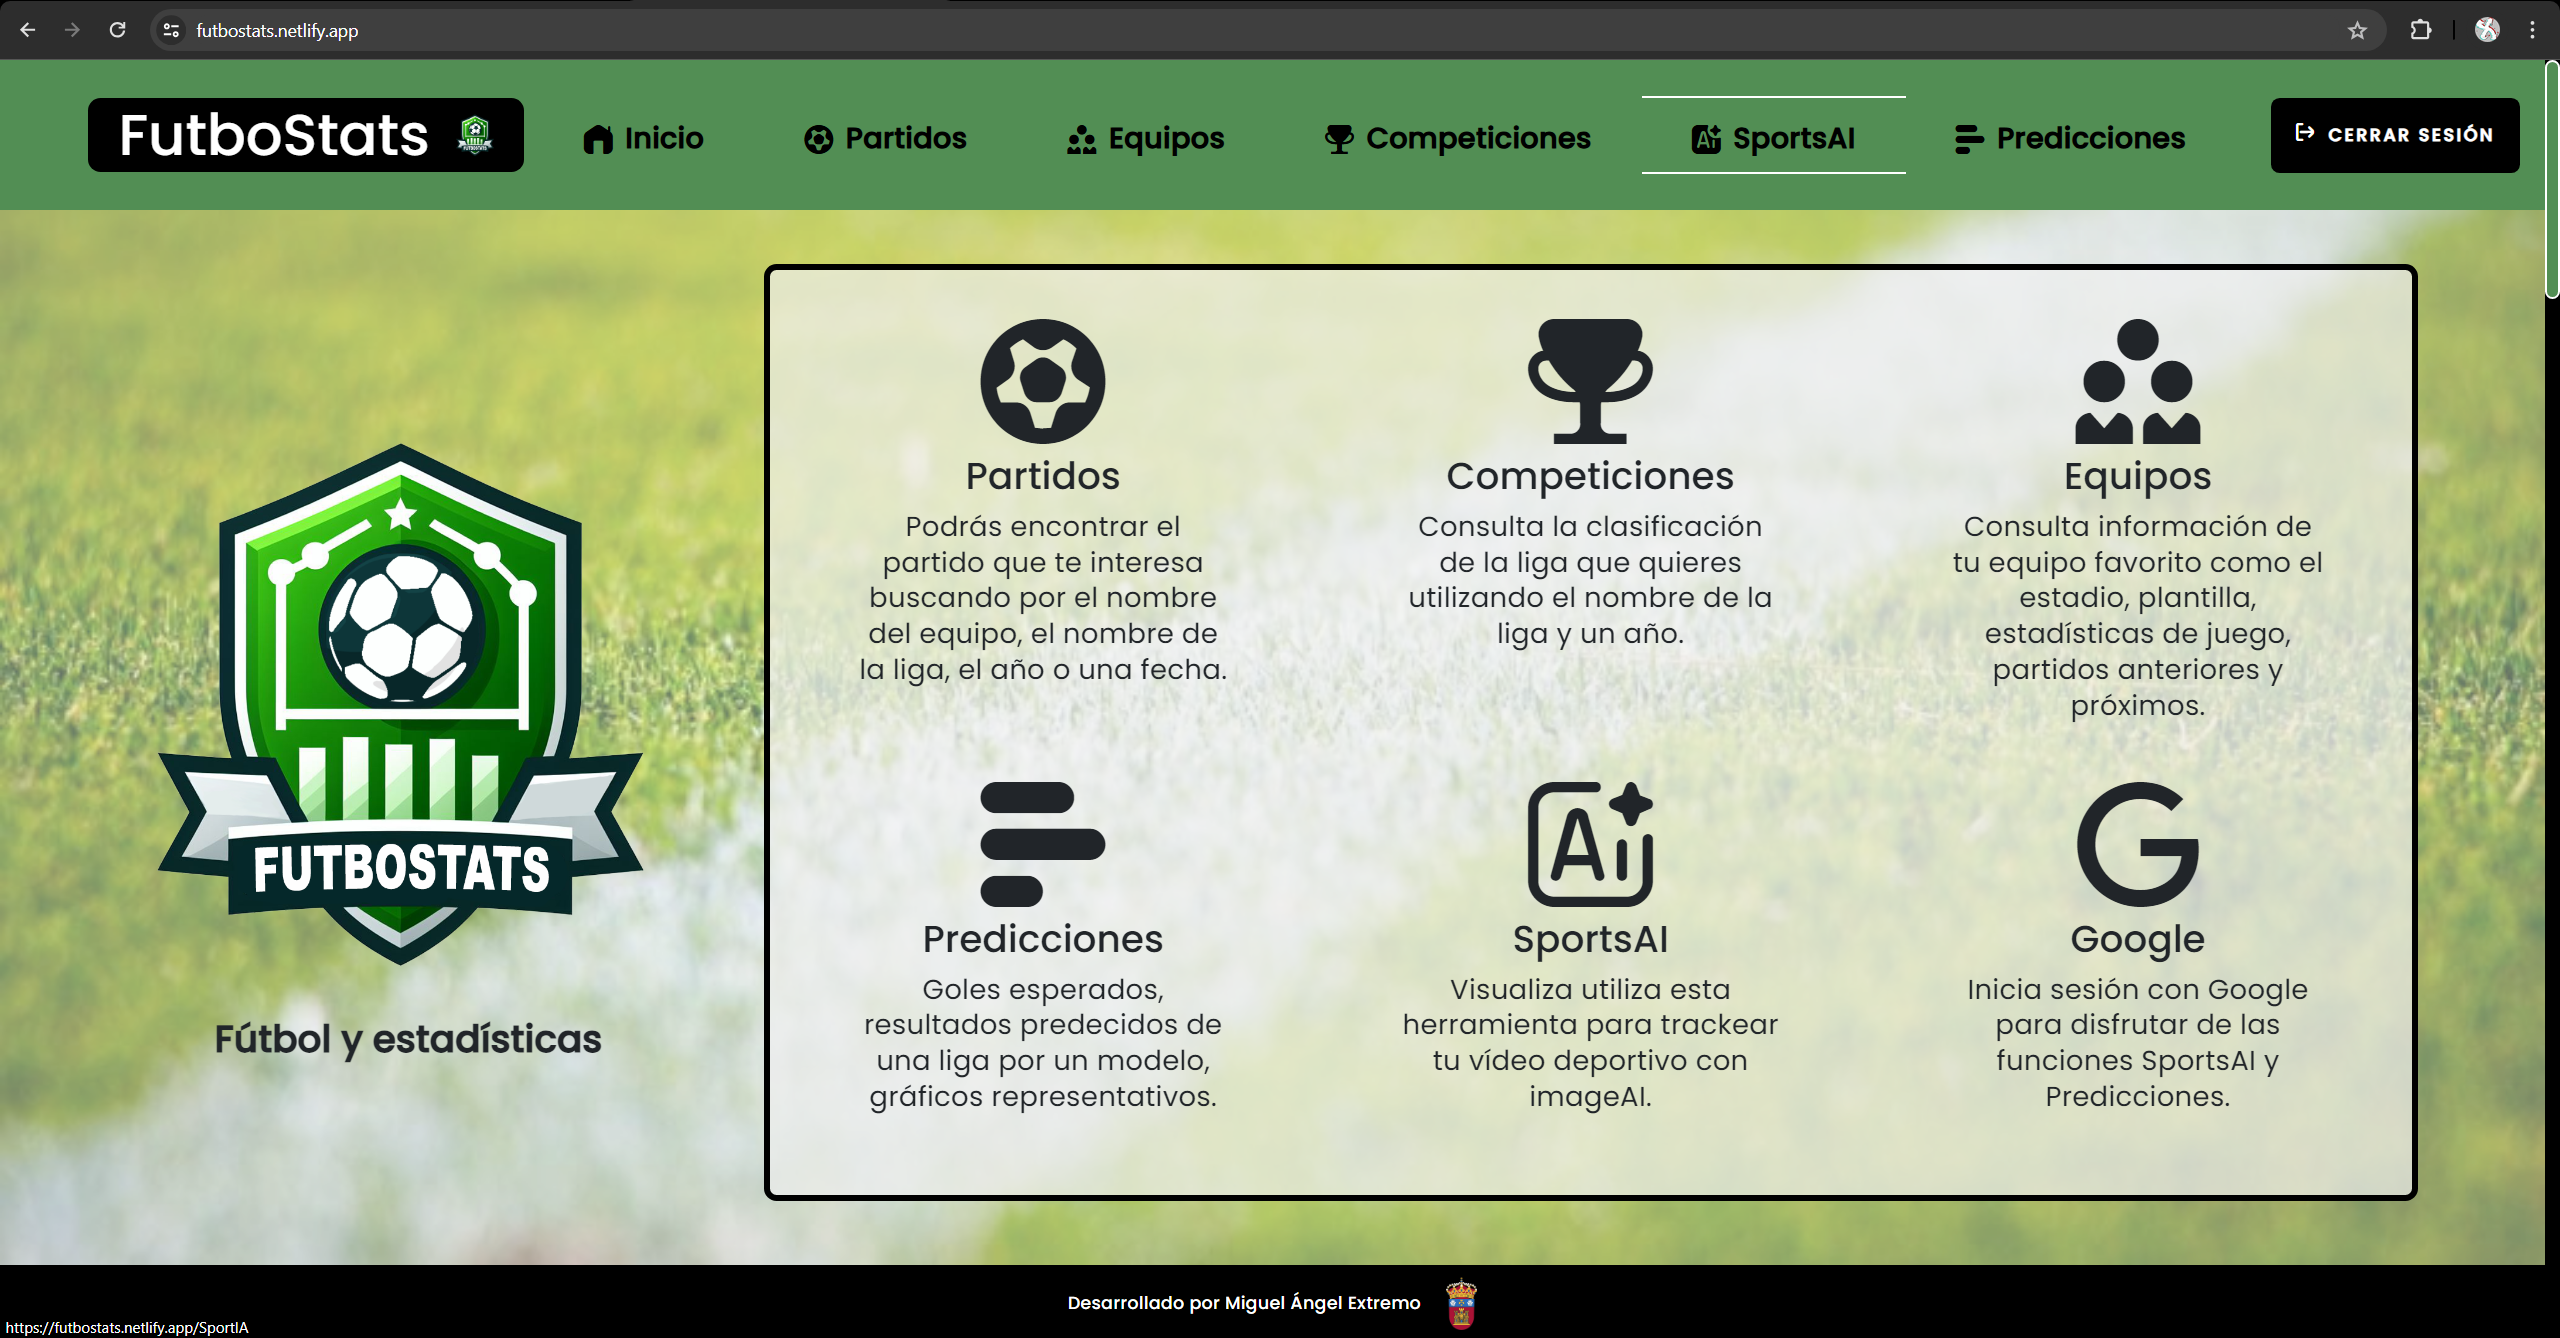
\includegraphics[width=1\linewidth]{img/iniciarSesion3-UM.png}
    \caption{Paso 3 de iniciar sesión en FutboStats: autenticado con éxito.}
    \label{fig:enter-label}
\end{figure}

\subsection{Cerrar sesión en FutboStats}
Si el usuario desea cerrar la sesión en FutboStats seguirá los siguientes pasos.
\begin{enumerate}
    \item Pulsar en el botón de 'Cerrar sesión'.
    \item Se mostrará una modal con dos opciones: cerrar sesión o cancelar.
    \item Si el usuario acepta cerrar sesión se cierra la sesión y no puede acceder a las funcionalidades protegidas de la aplicación.
    \item Si el usuario cancela cerrar sesión puede seguir accediendo a las funcionalidades protegidas de la aplicación.
\end{enumerate}
\begin{figure}[H]
    \centering
    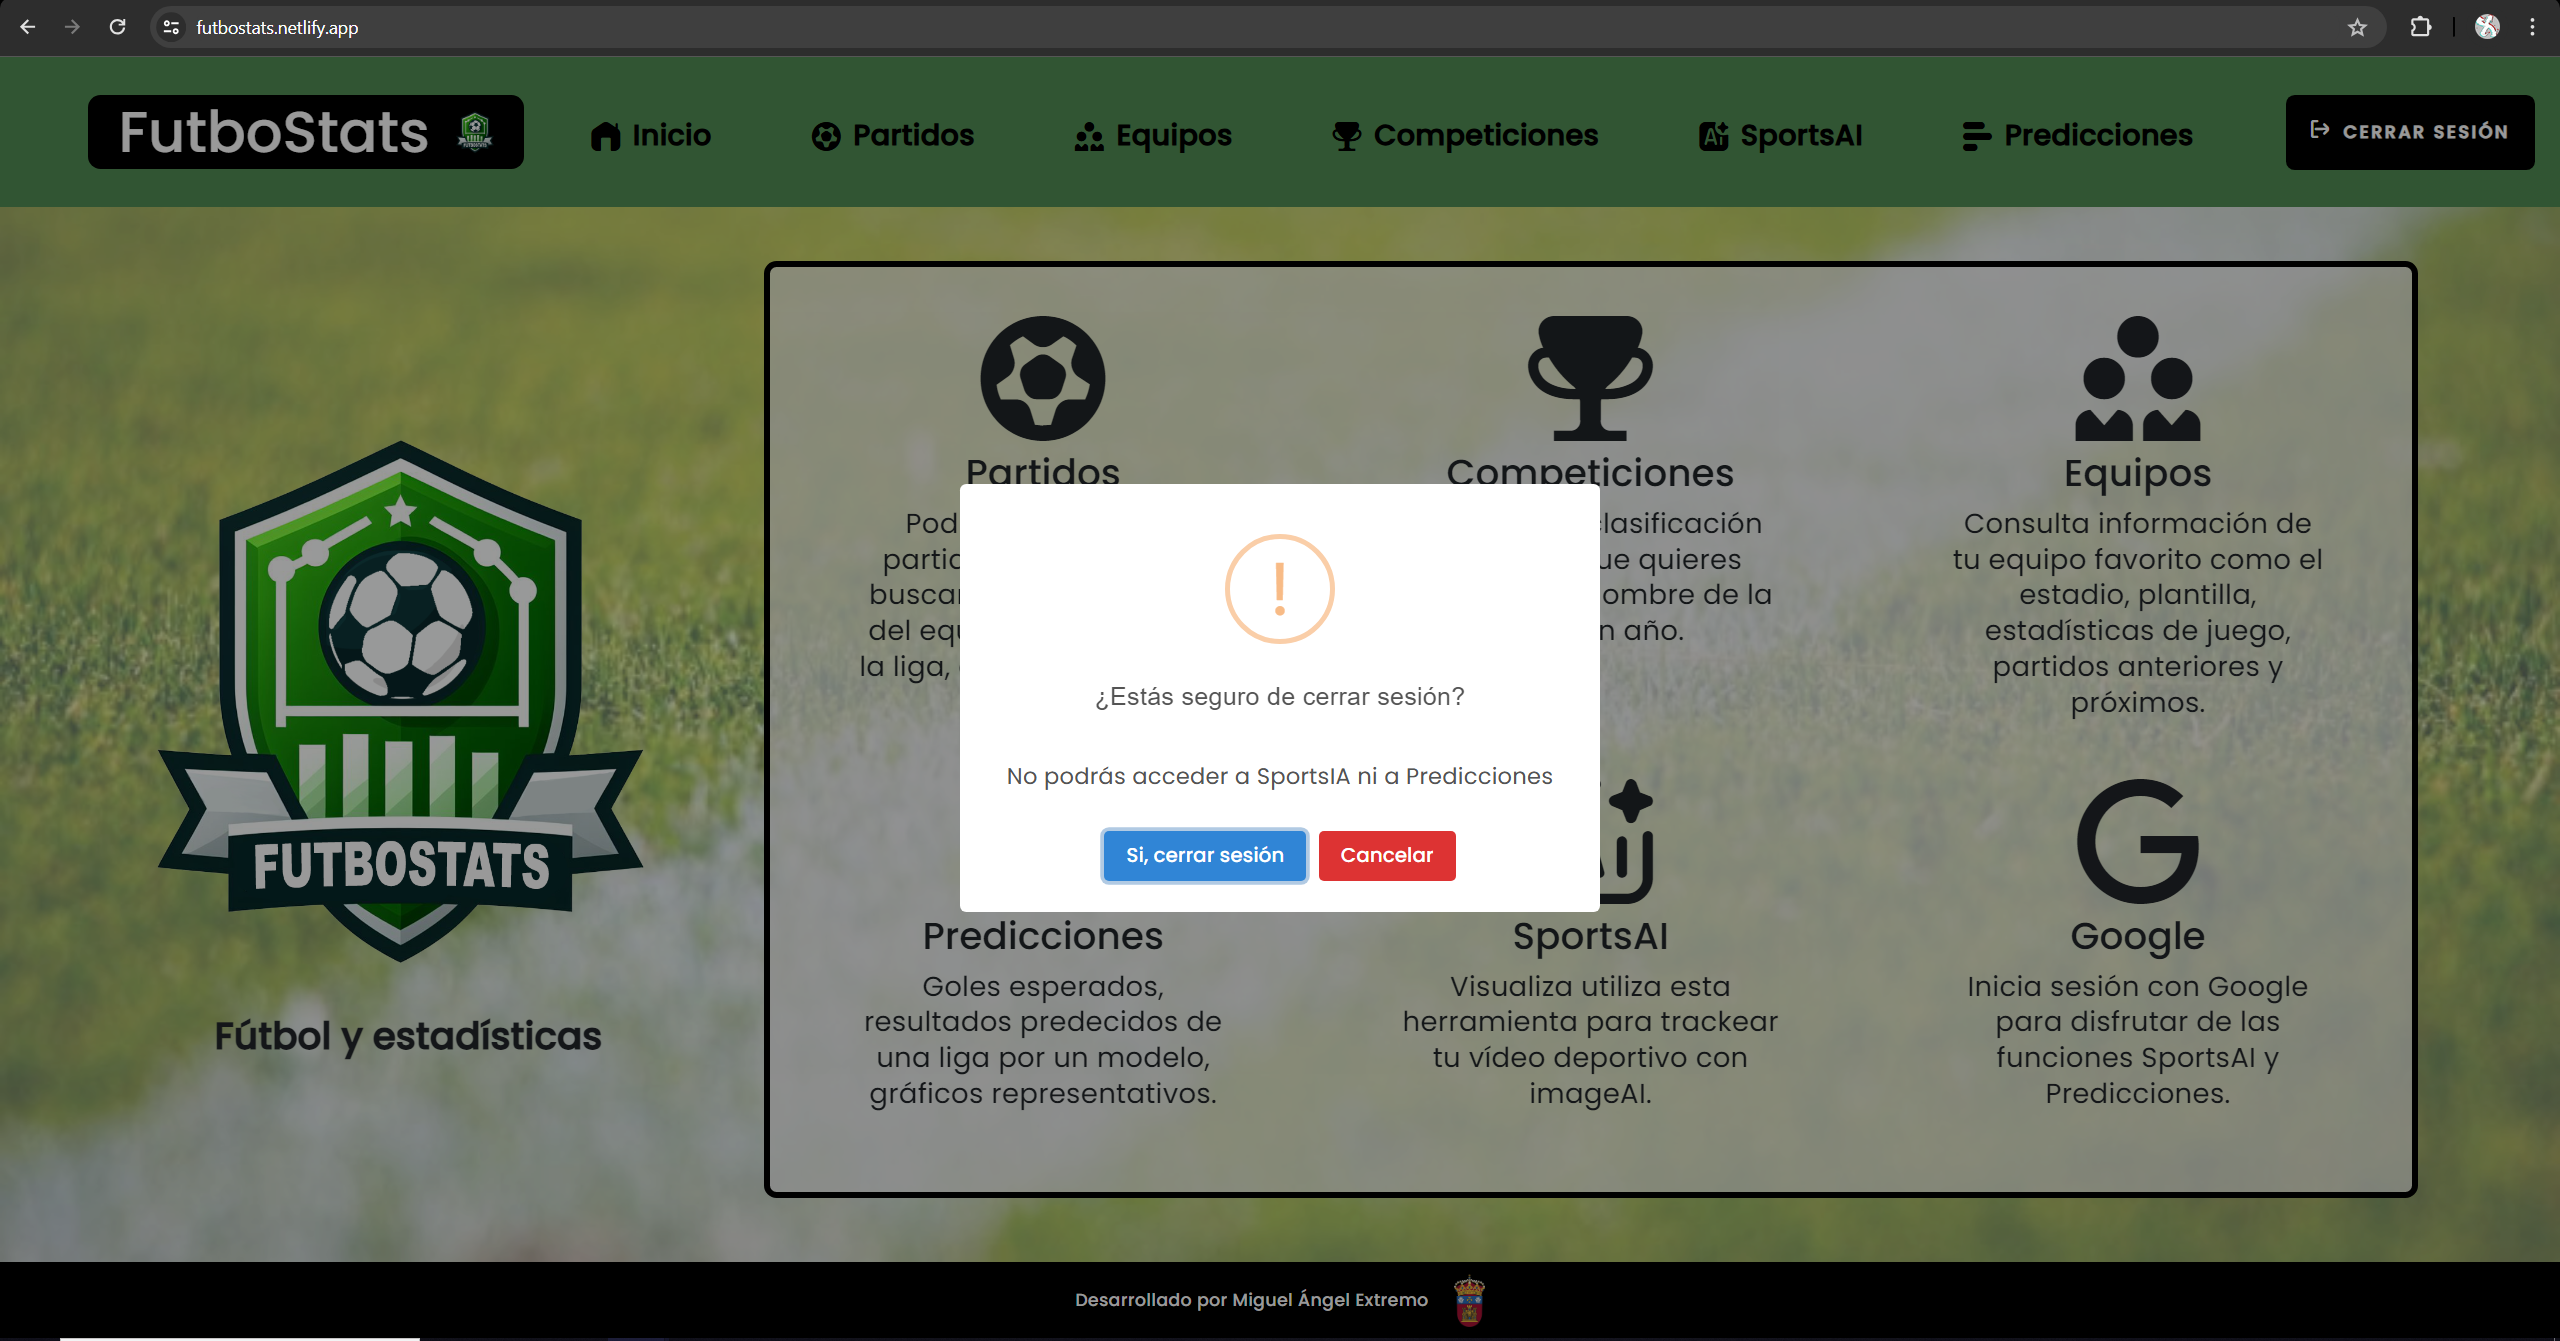
\includegraphics[width=1\linewidth]{img/cerrarSesion-UM.png}
    \caption{Cerrar sesión en FutboStats.}
    \label{fig:enter-label}
\end{figure}

\subsection{Utilizar SportAI en FutboStats}
En la opción 'SportsAI' de FutboStats el usuario podrá subir un vídeo suyo en la aplicación y obtener un vídeo con el procesado de imageAI. \\
Los pasos que debe seguir para utilizar esta funcionalidad son:
\begin{enumerate}
    \item Iniciar sesión en la aplicación.
    \item Pulsar en la opción 'SportsAI' del menú superior.
    \item Hacer click para elegir o arrastrar un vídeo en formato '.mp4'.
    \item Esperar a que la aplicación genere el vídeo procesado por imageAI.
    \item El usuario podrá visualizar el vídeo nuevo en la aplicación.
\end{enumerate}

\begin{figure}[H]
    \centering
    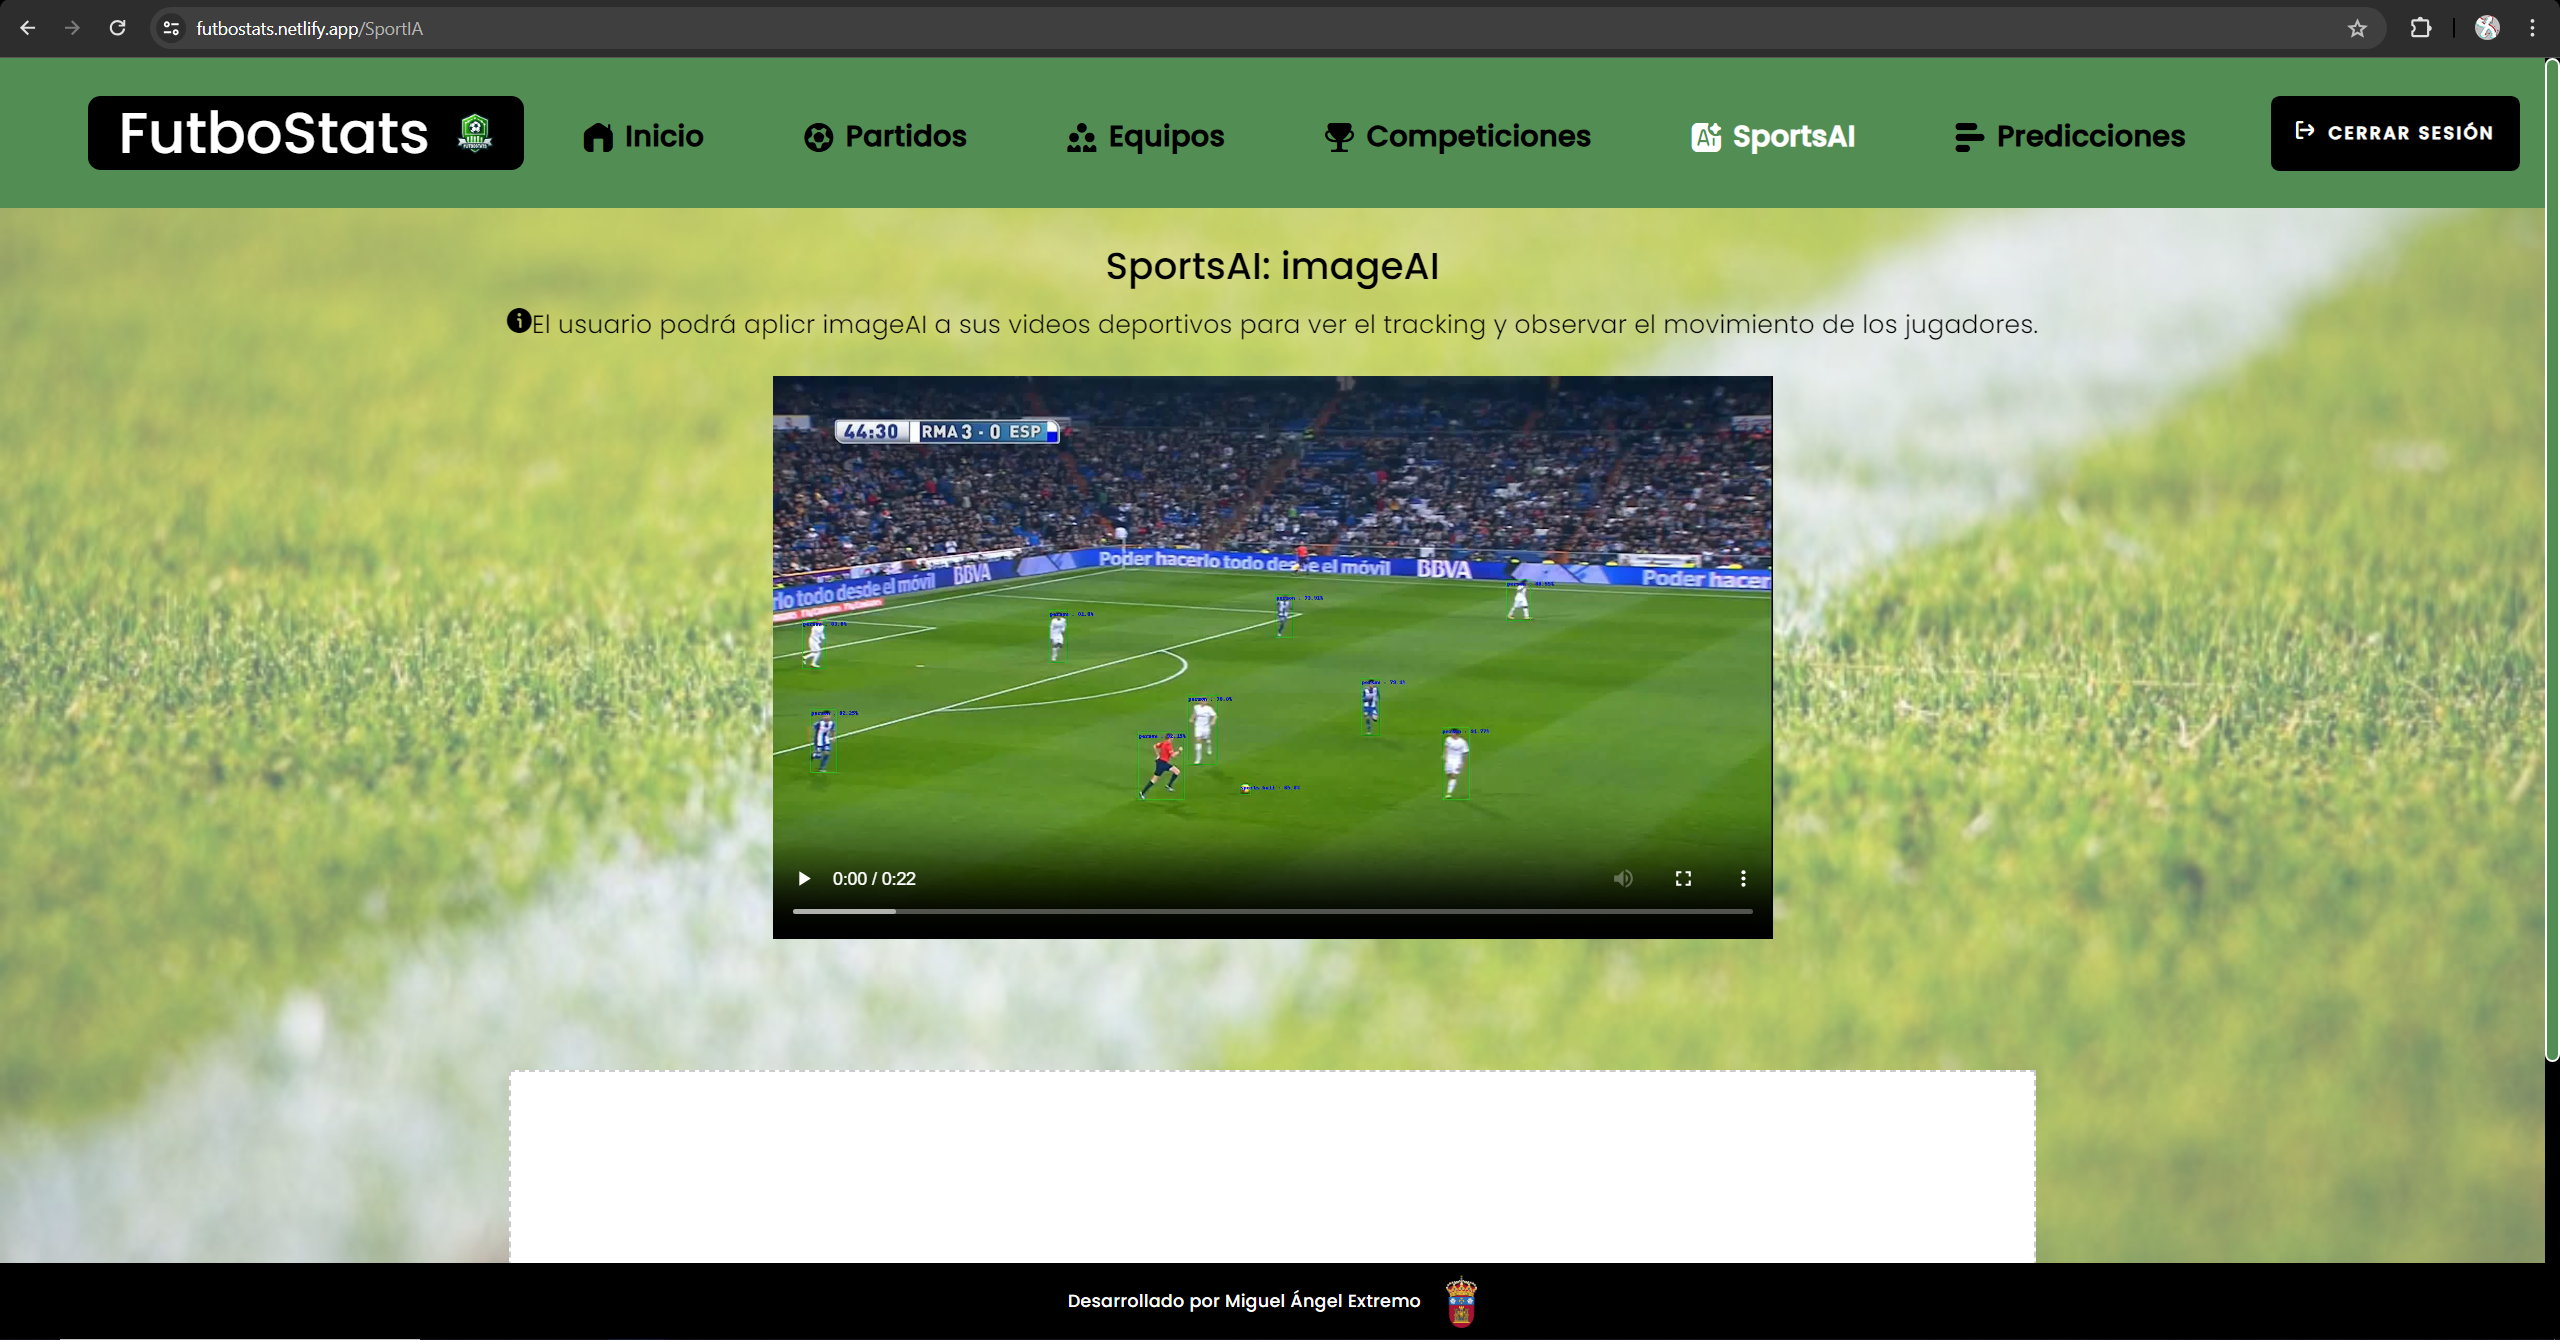
\includegraphics[width=1\linewidth]{img/sportsAI-UM.png}
    \caption{Paso 1 para utilizar SportAI: entrar en 'SportsAI'.}
    \label{fig:enter-label}
\end{figure}

\begin{figure}[H]
    \centering
    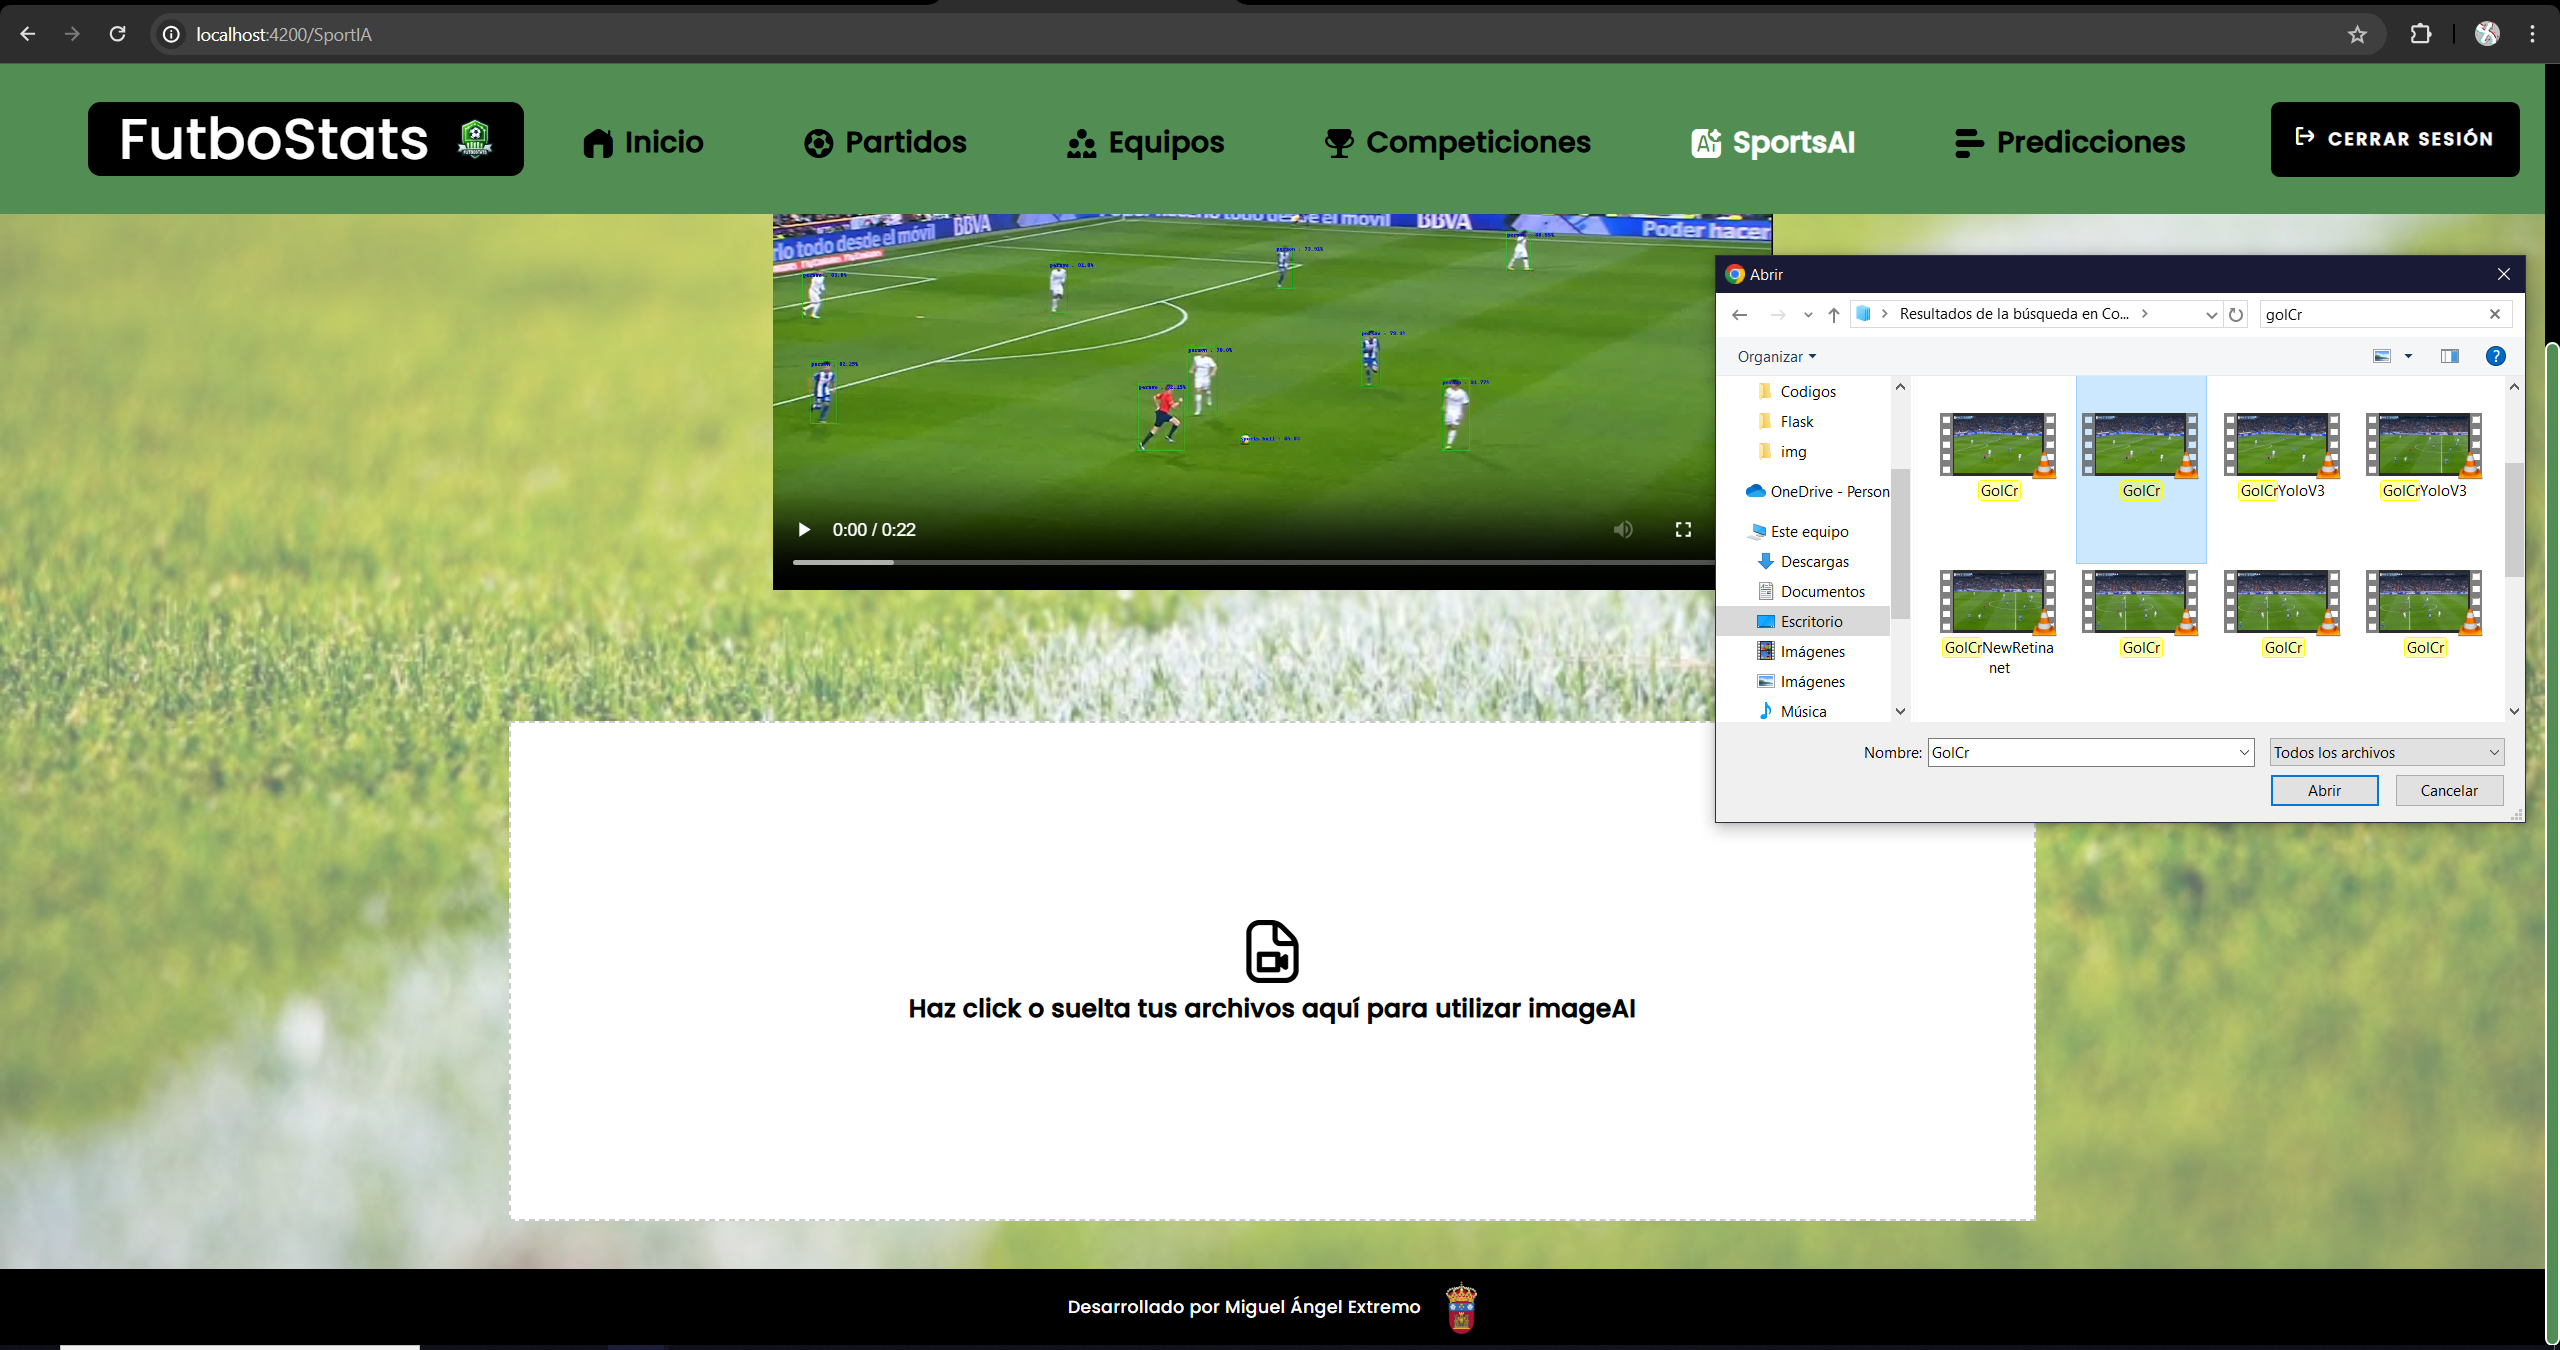
\includegraphics[width=1\linewidth]{img/sportsAI2-UM.png}
    \caption{Paso 2 para utilizar SportAI: pulsar o arrastrar un vídeo '.mp4'.}
    \label{fig:enter-label}
\end{figure}

\begin{figure}[H]
    \centering
    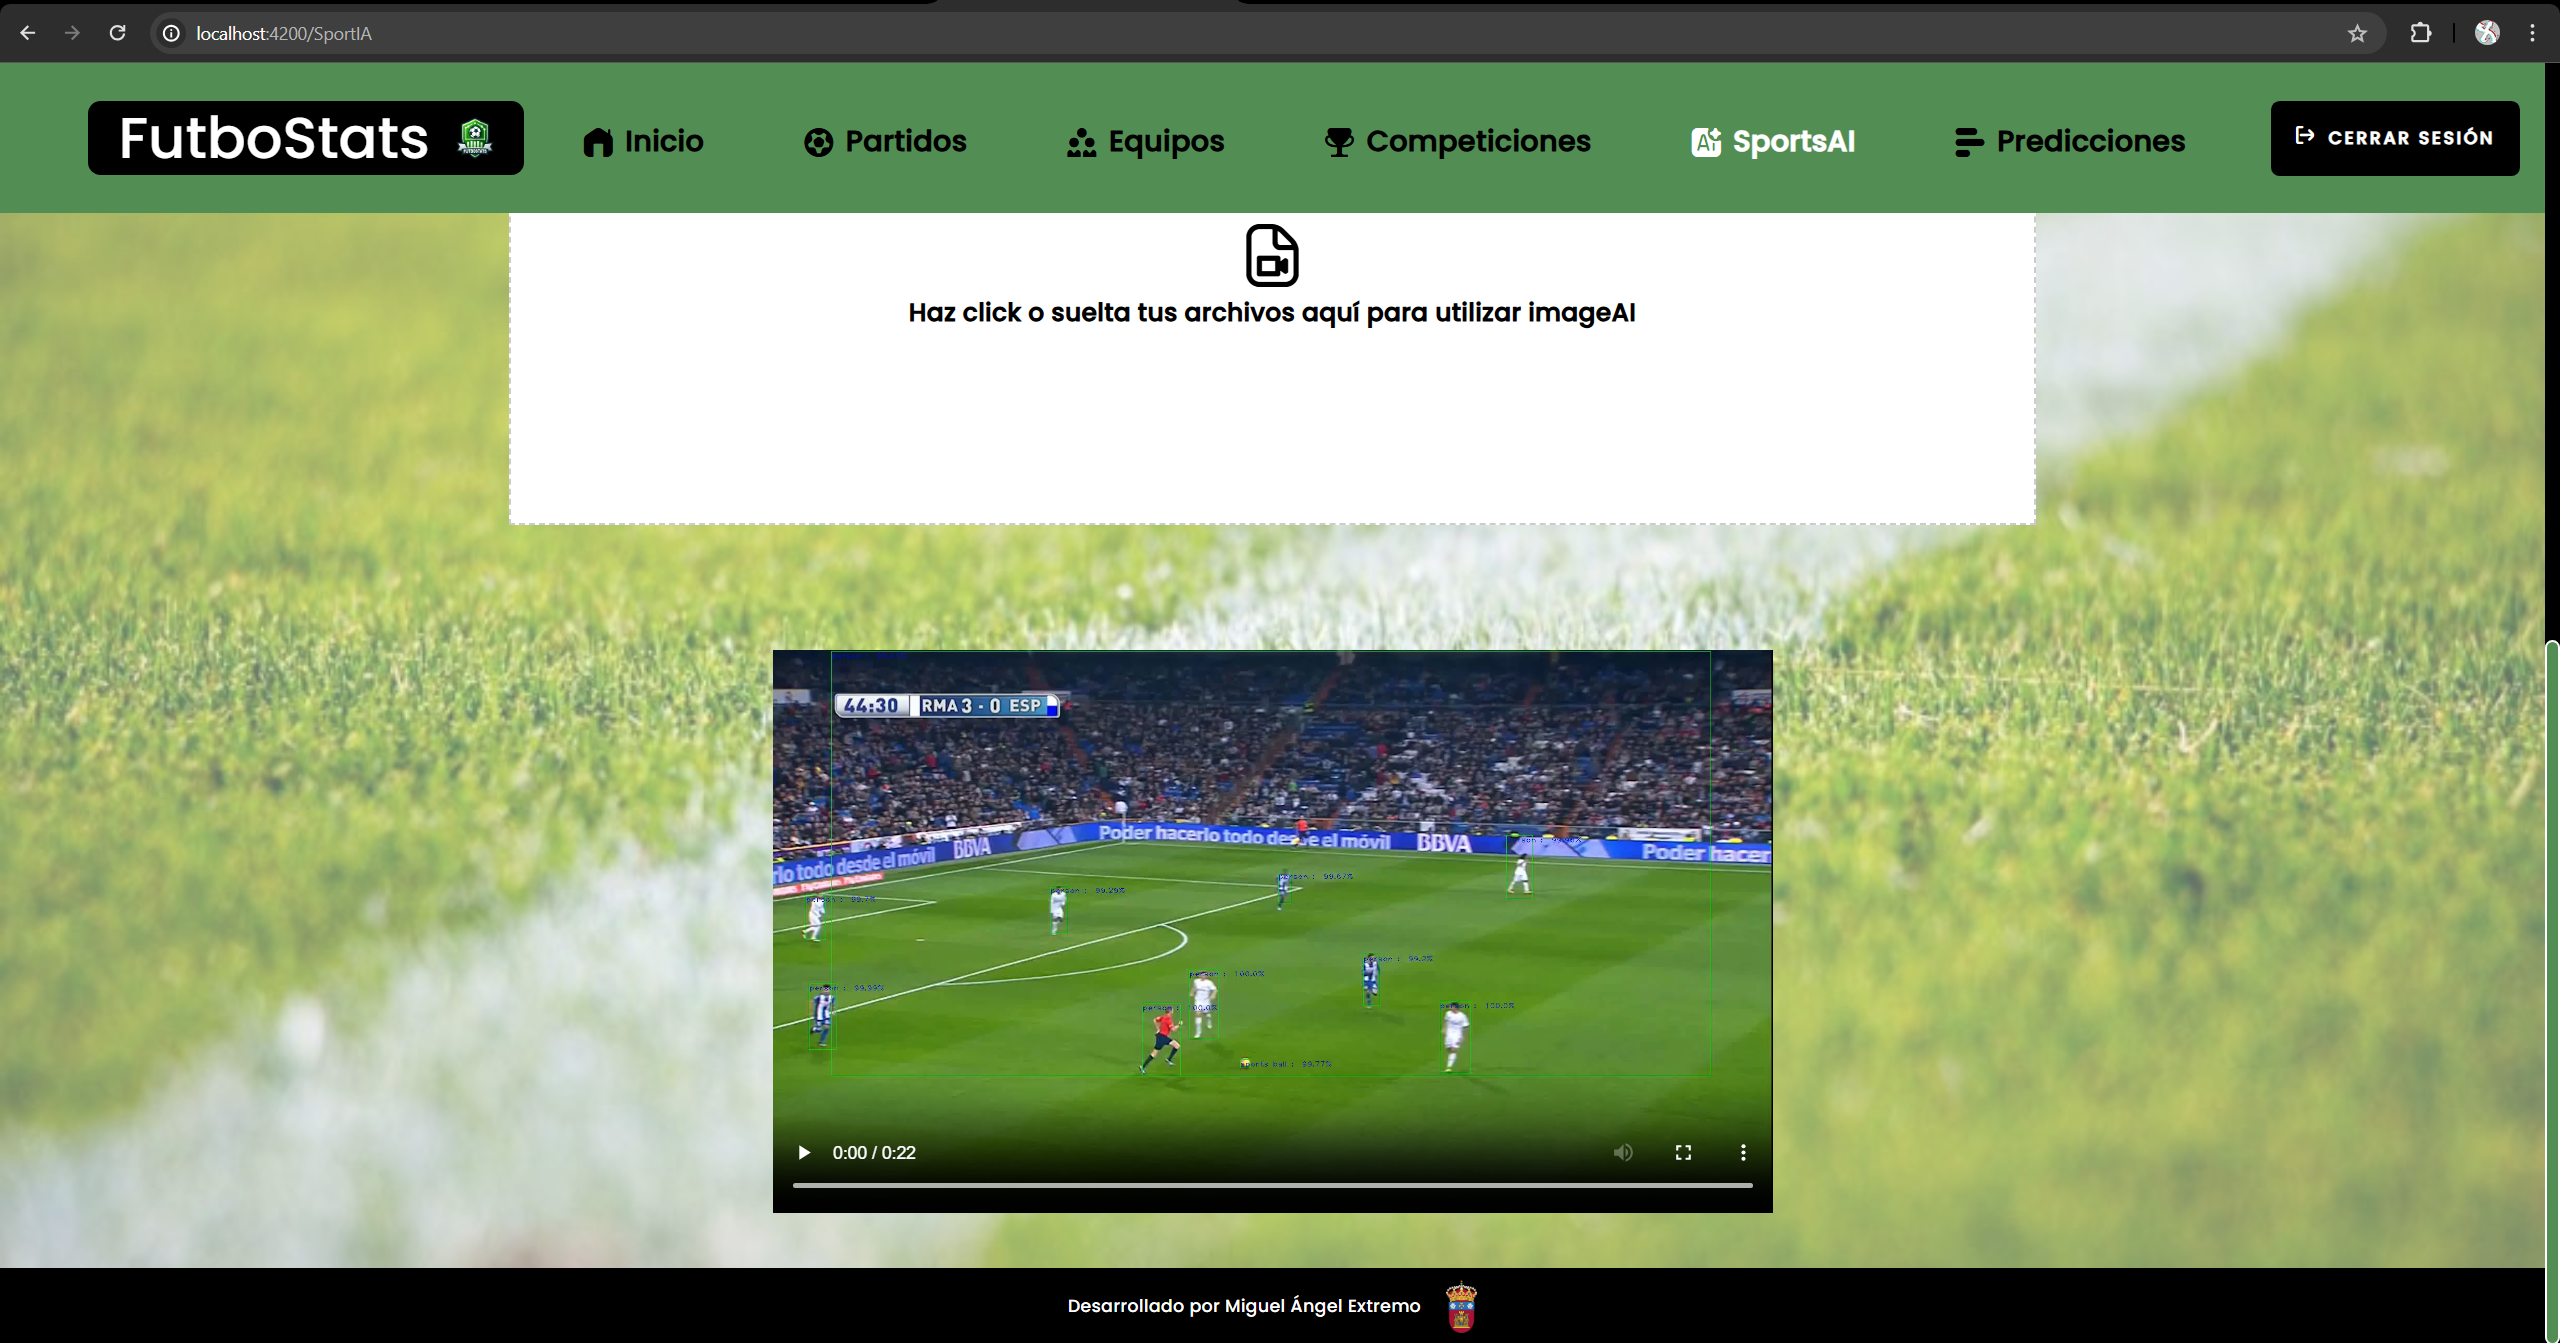
\includegraphics[width=1\linewidth]{img/sportsAI3-UM.png}
    \caption{Paso 3 para utilizar SportAI: visualizar el vídeo generado por imageAI}
    \label{fig:enter-label}
\end{figure}

\subsection{Utilizar Predicciones en FutboStats}
En la opción 'Predicciones' de FutboStats el usuario podrá consultar predicciones, modelo de goles esperados, puntos esperados y gráficas de estadísticas del mundial de una forma sencilla. \\
Los pasos a seguir son:
\begin{enumerate}
    \item Iniciar sesión en la aplicación.
    \item Pulsar en la opción 'Predicciones' del menú superior.
    \item El usuario accede a clasificaciones y puede visualizar una comparación entre la tabla de puntos esperados generada por el modelo y la clasificación real. Además, puede visualizar un gráfico que muestra el desarrollo de los equipos en la liga a lo largo de las jornadas. Las ligas disponibles son La Liga, Bundesliga, Premier League, Serie A y Ligue1. Los datos pertenecen a la temporada 2015/2016.
    \item El usuario puede pulsar en el menú secundario y acceder a 'Goles esperados xG'. El usuario puede visualizar los resultados del modelo mediante tablas y gráficas. Si el usuario hace click o pone el cursor encima de las tarjetas podrá leer información acerca de las representaciones gráficas.
    \item El usuario puede pulsar en el menú secundario y accedera 'Mundial'. El usuario puede visualizar gráficos que representan estadísticas de la final del mundial de 2022 entre Francia y Argentina. El usuario puede elegir el gráfico que quiere visualizar eligiendo el jugador que prefiera. Si el usuario hace click o pone el cursor encima de la tarjeta podrá leer información acerca de las representaciones gráficas.
\end{enumerate}

\begin{figure}[H]
    \centering
    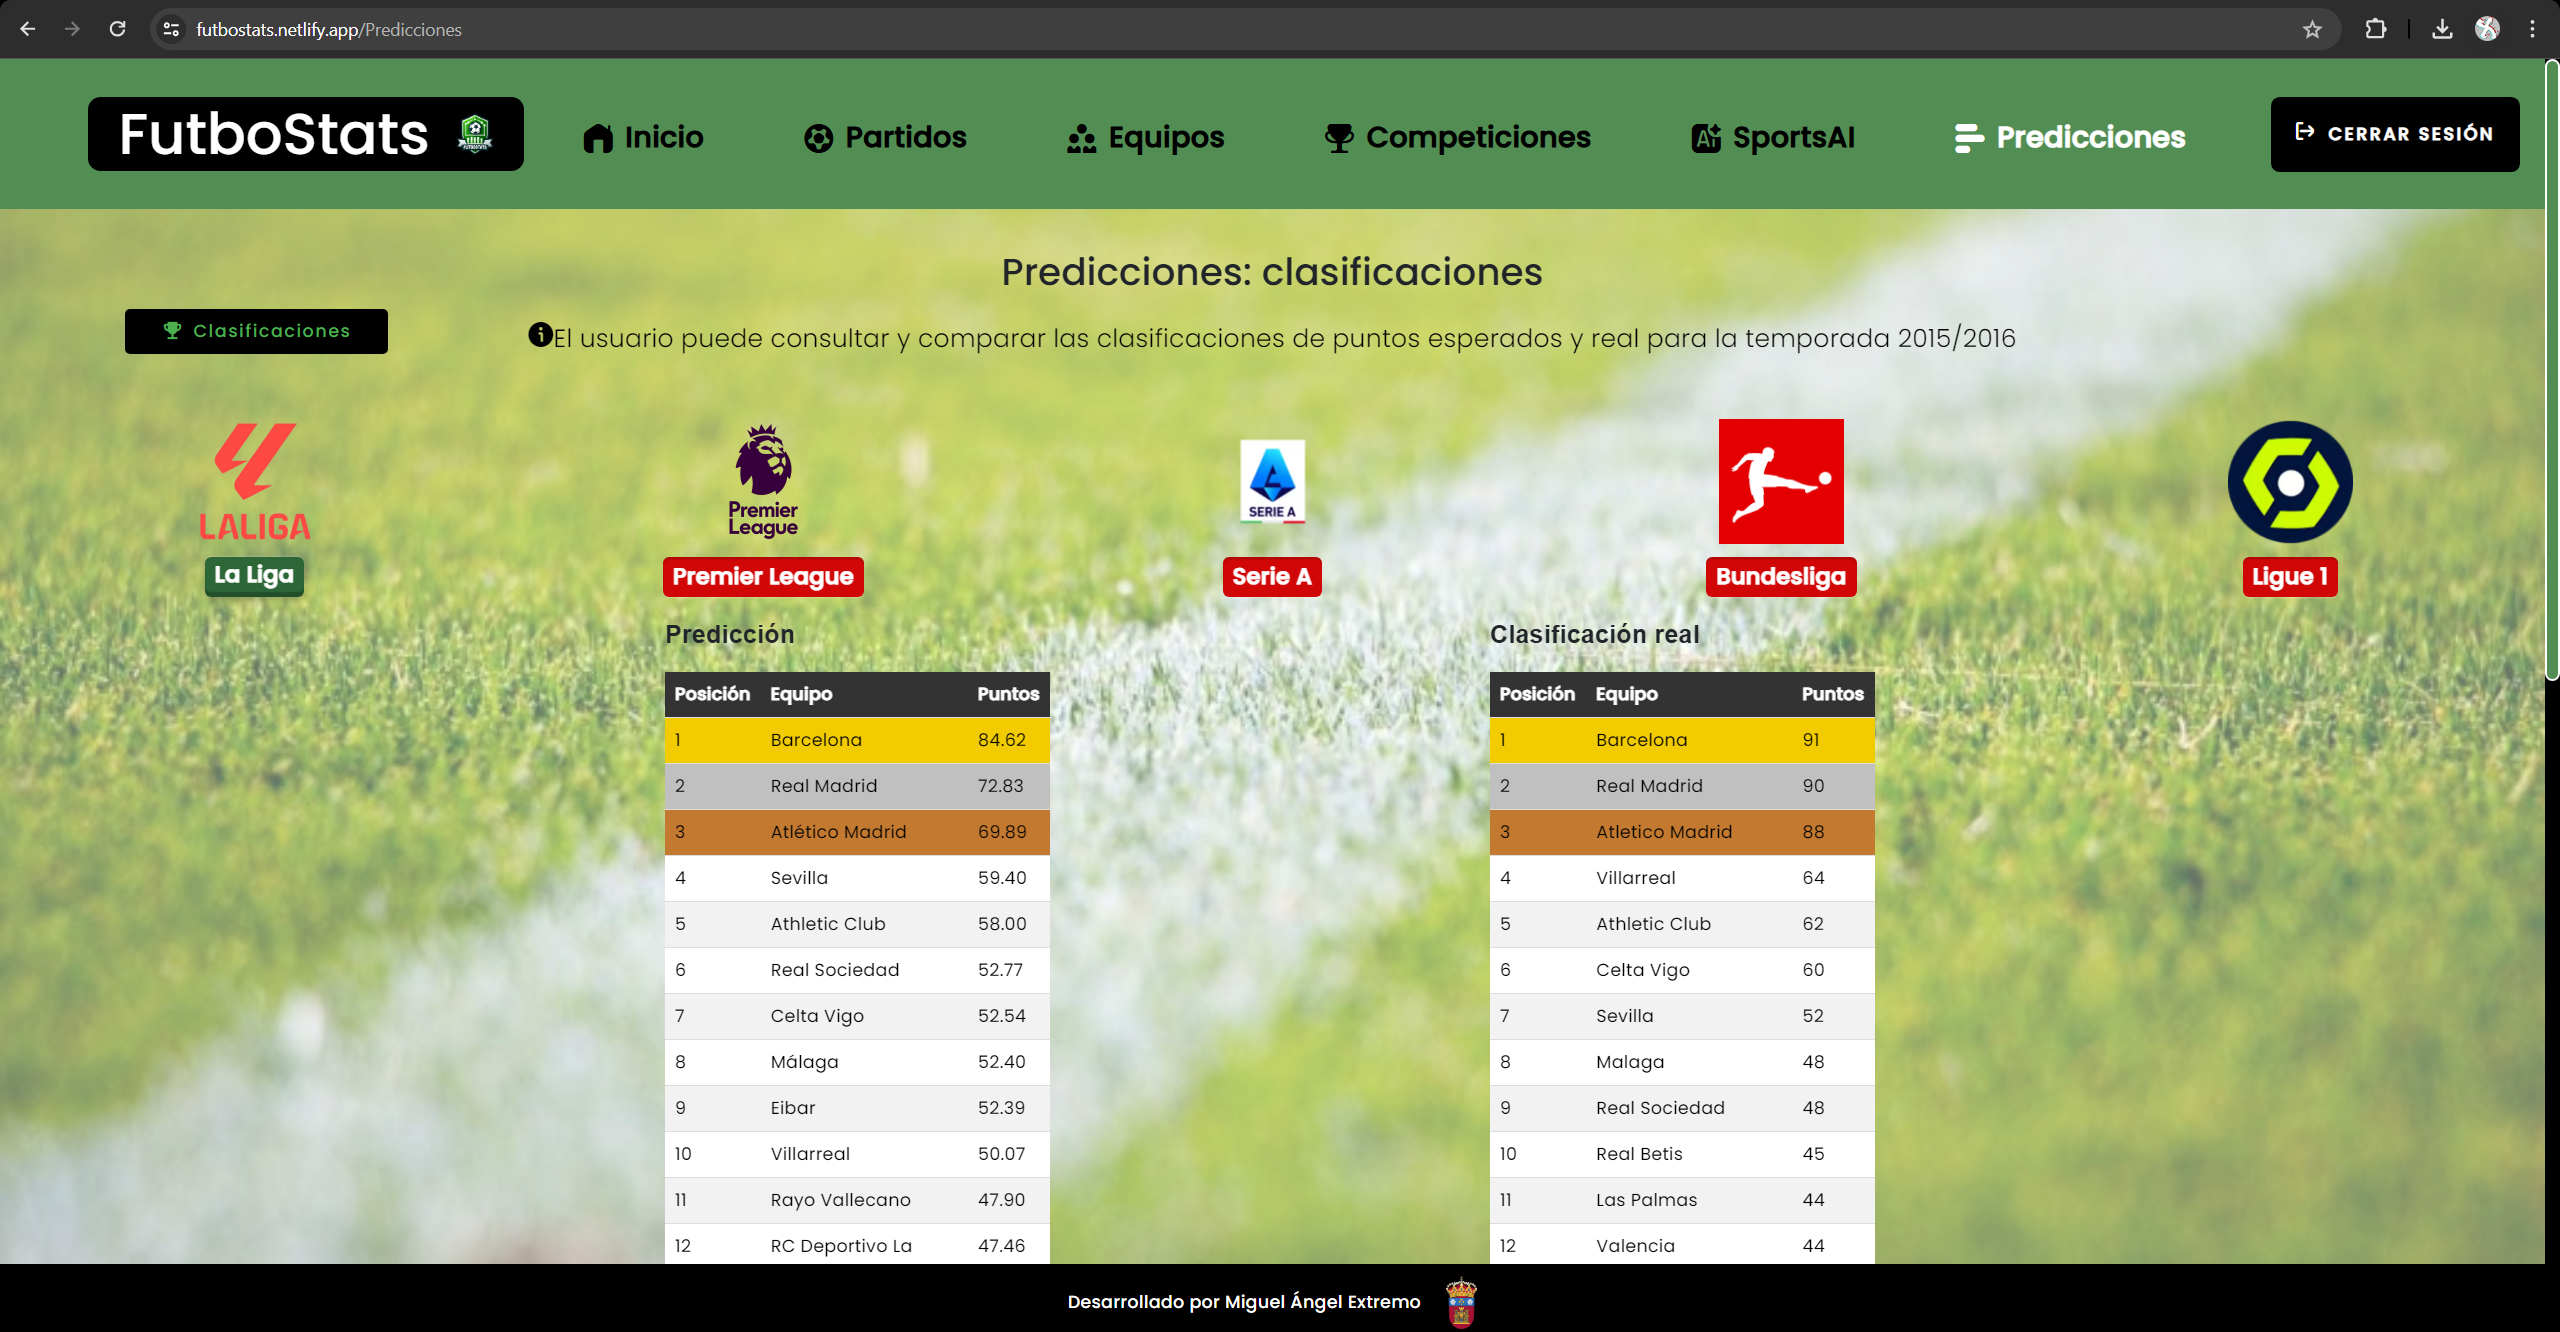
\includegraphics[width=1\linewidth]{img/predicciones1-UM.png}
    \caption{Visualización de predicción de puntos esperados y real.}
    \label{fig:enter-label}
\end{figure}

\begin{figure}[H]
    \centering
    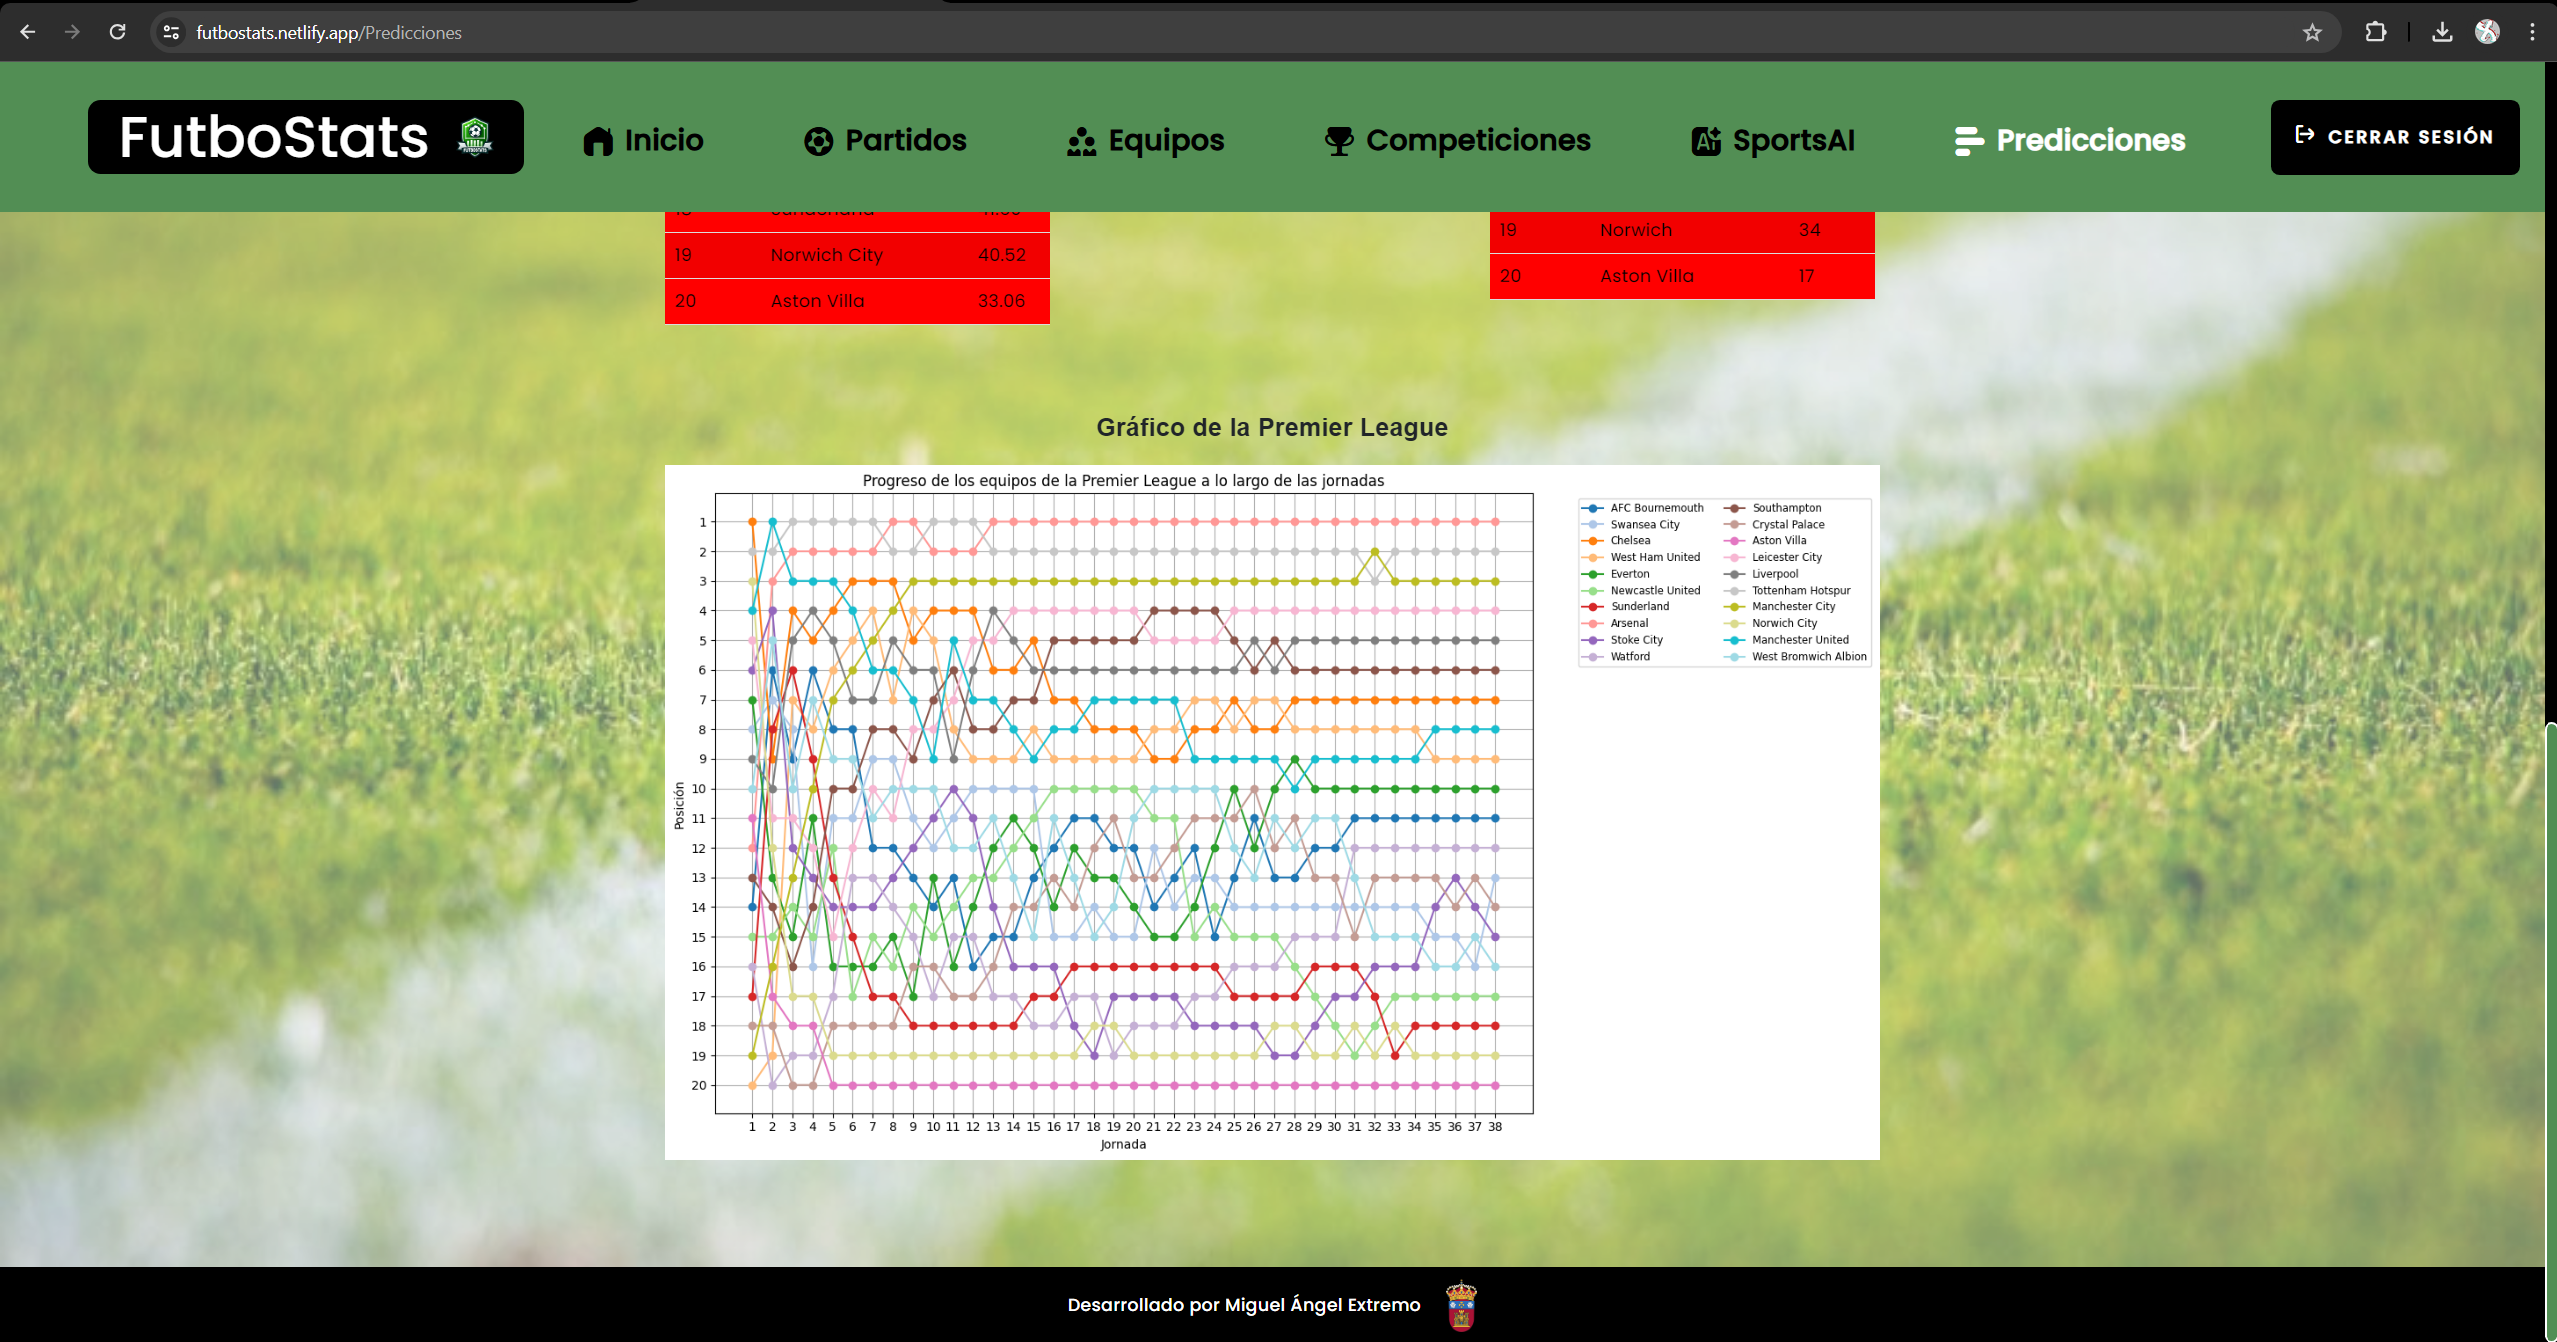
\includegraphics[width=1\linewidth]{img/predicciones2-UM.png}
    \caption{Representación gráfica de los puntos esperados a lo largo de las jornadas.}
    \label{fig:enter-label}
\end{figure}

\begin{figure}[H]
    \centering
    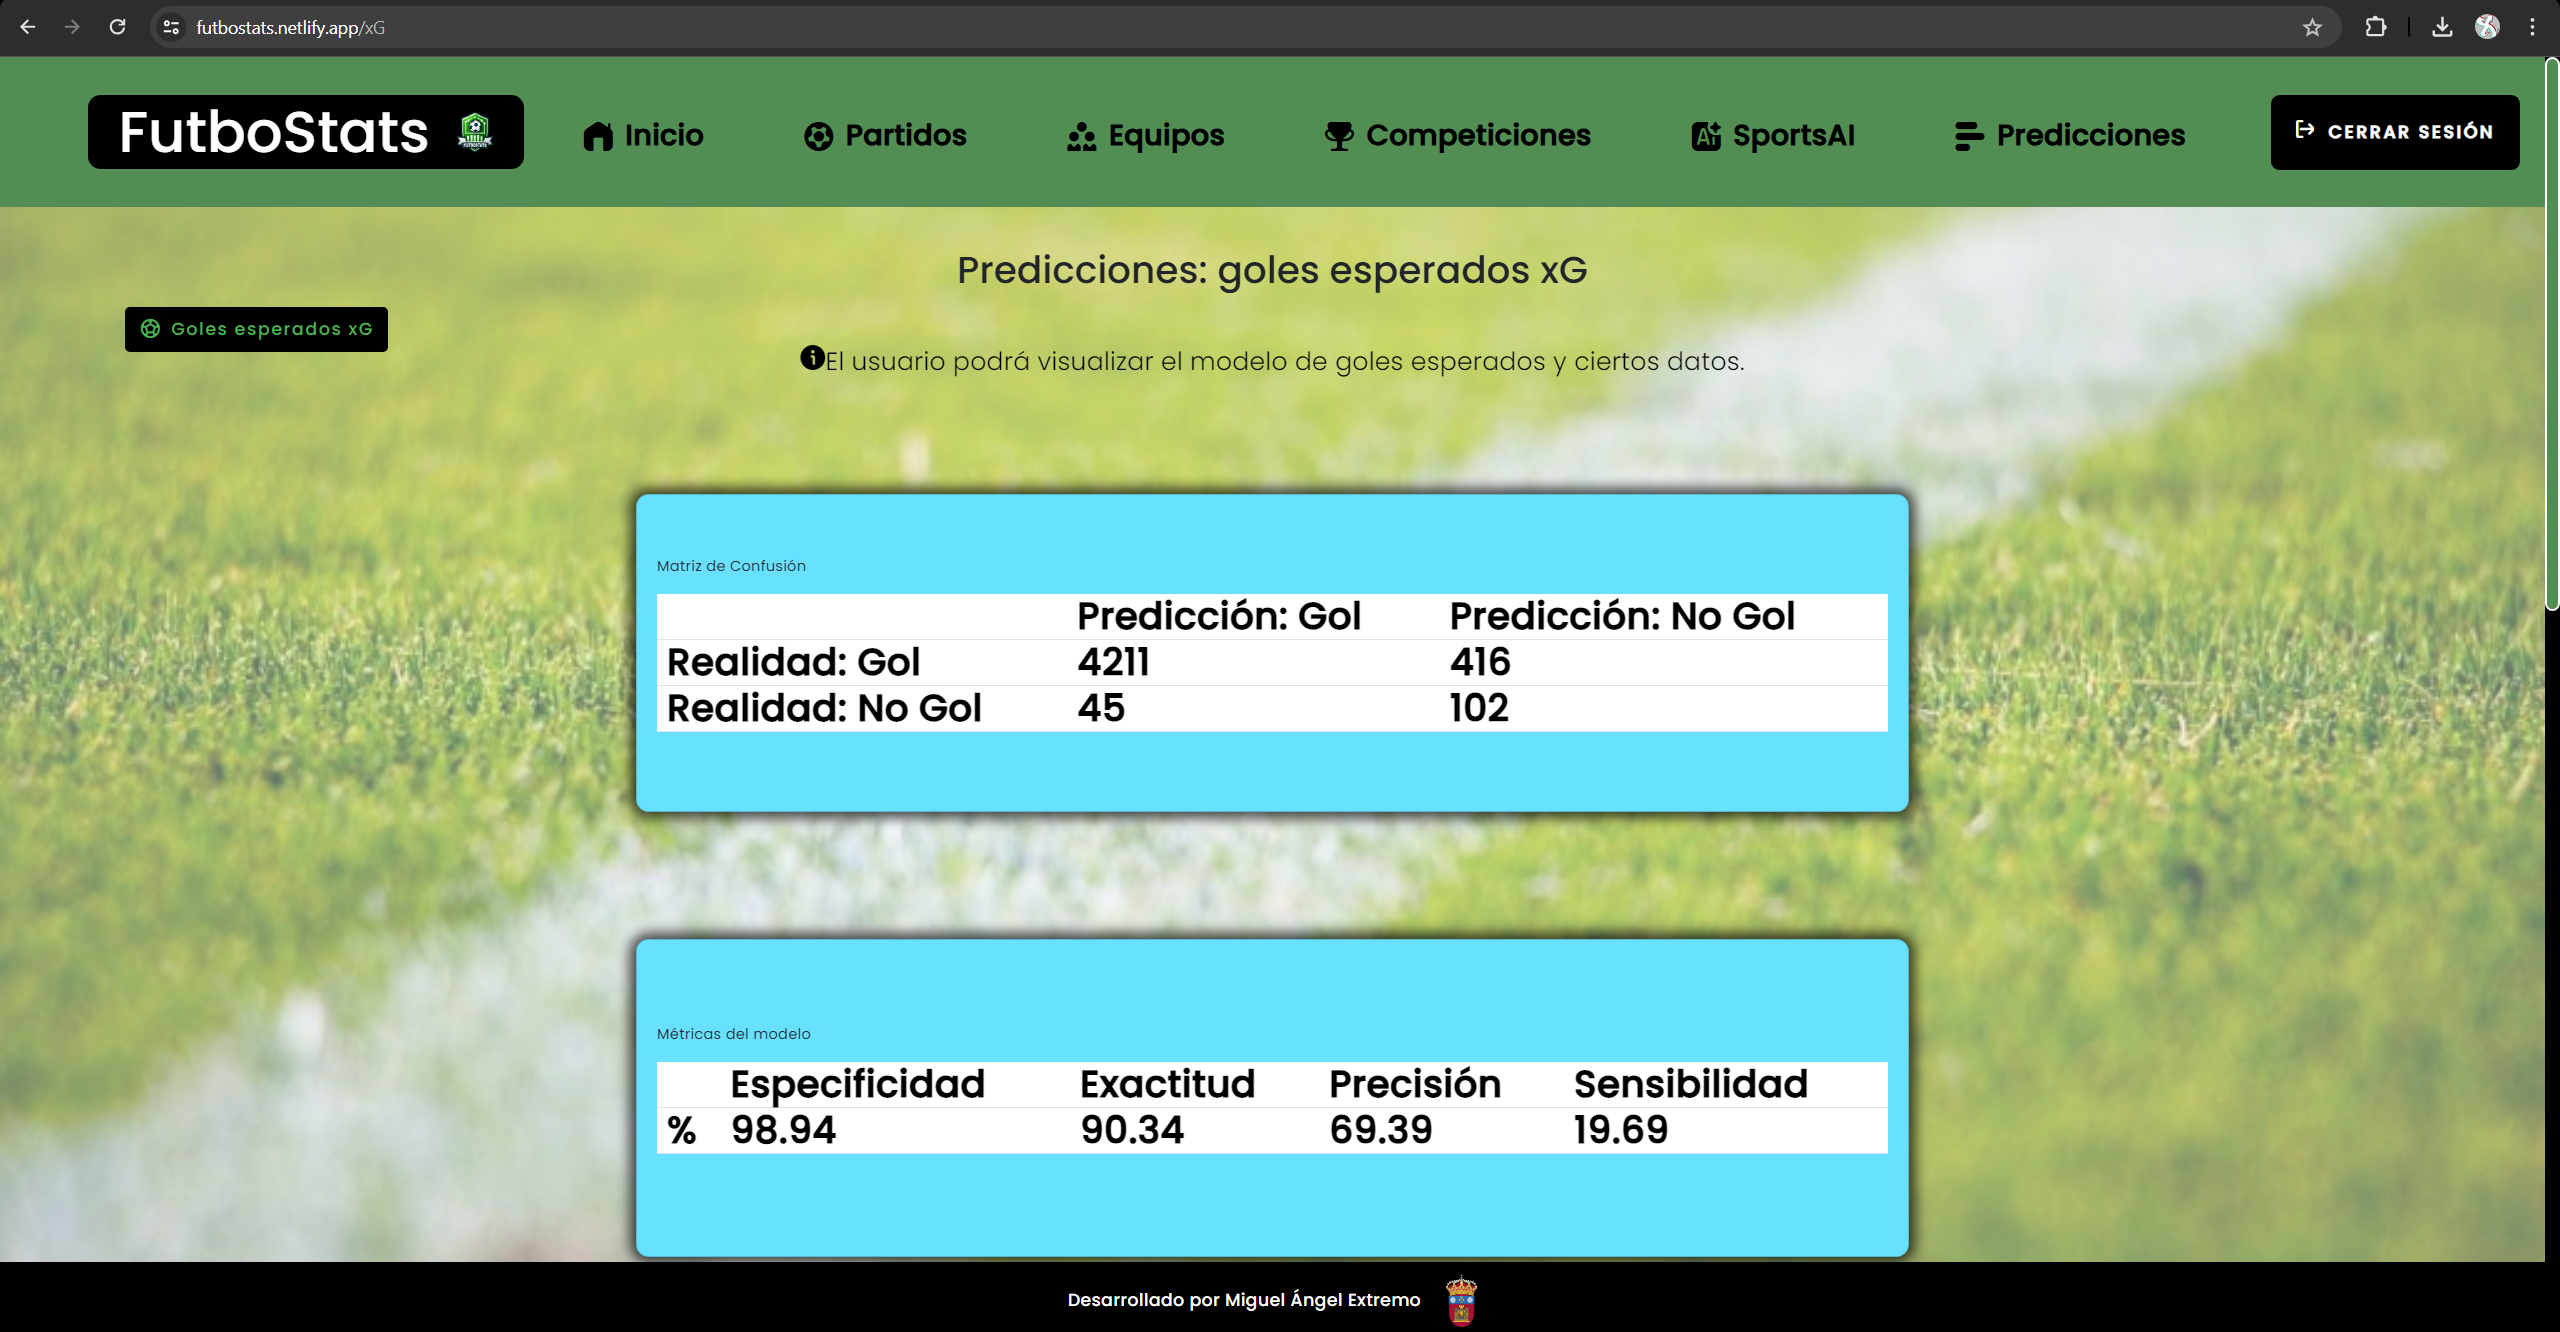
\includegraphics[width=1\linewidth]{img/golesEsperados1-UM.png}
    \caption{Visualización tablas del modelo de goles esperados xG}
    \label{fig:enter-label}
\end{figure}

\begin{figure}[H]
    \centering
    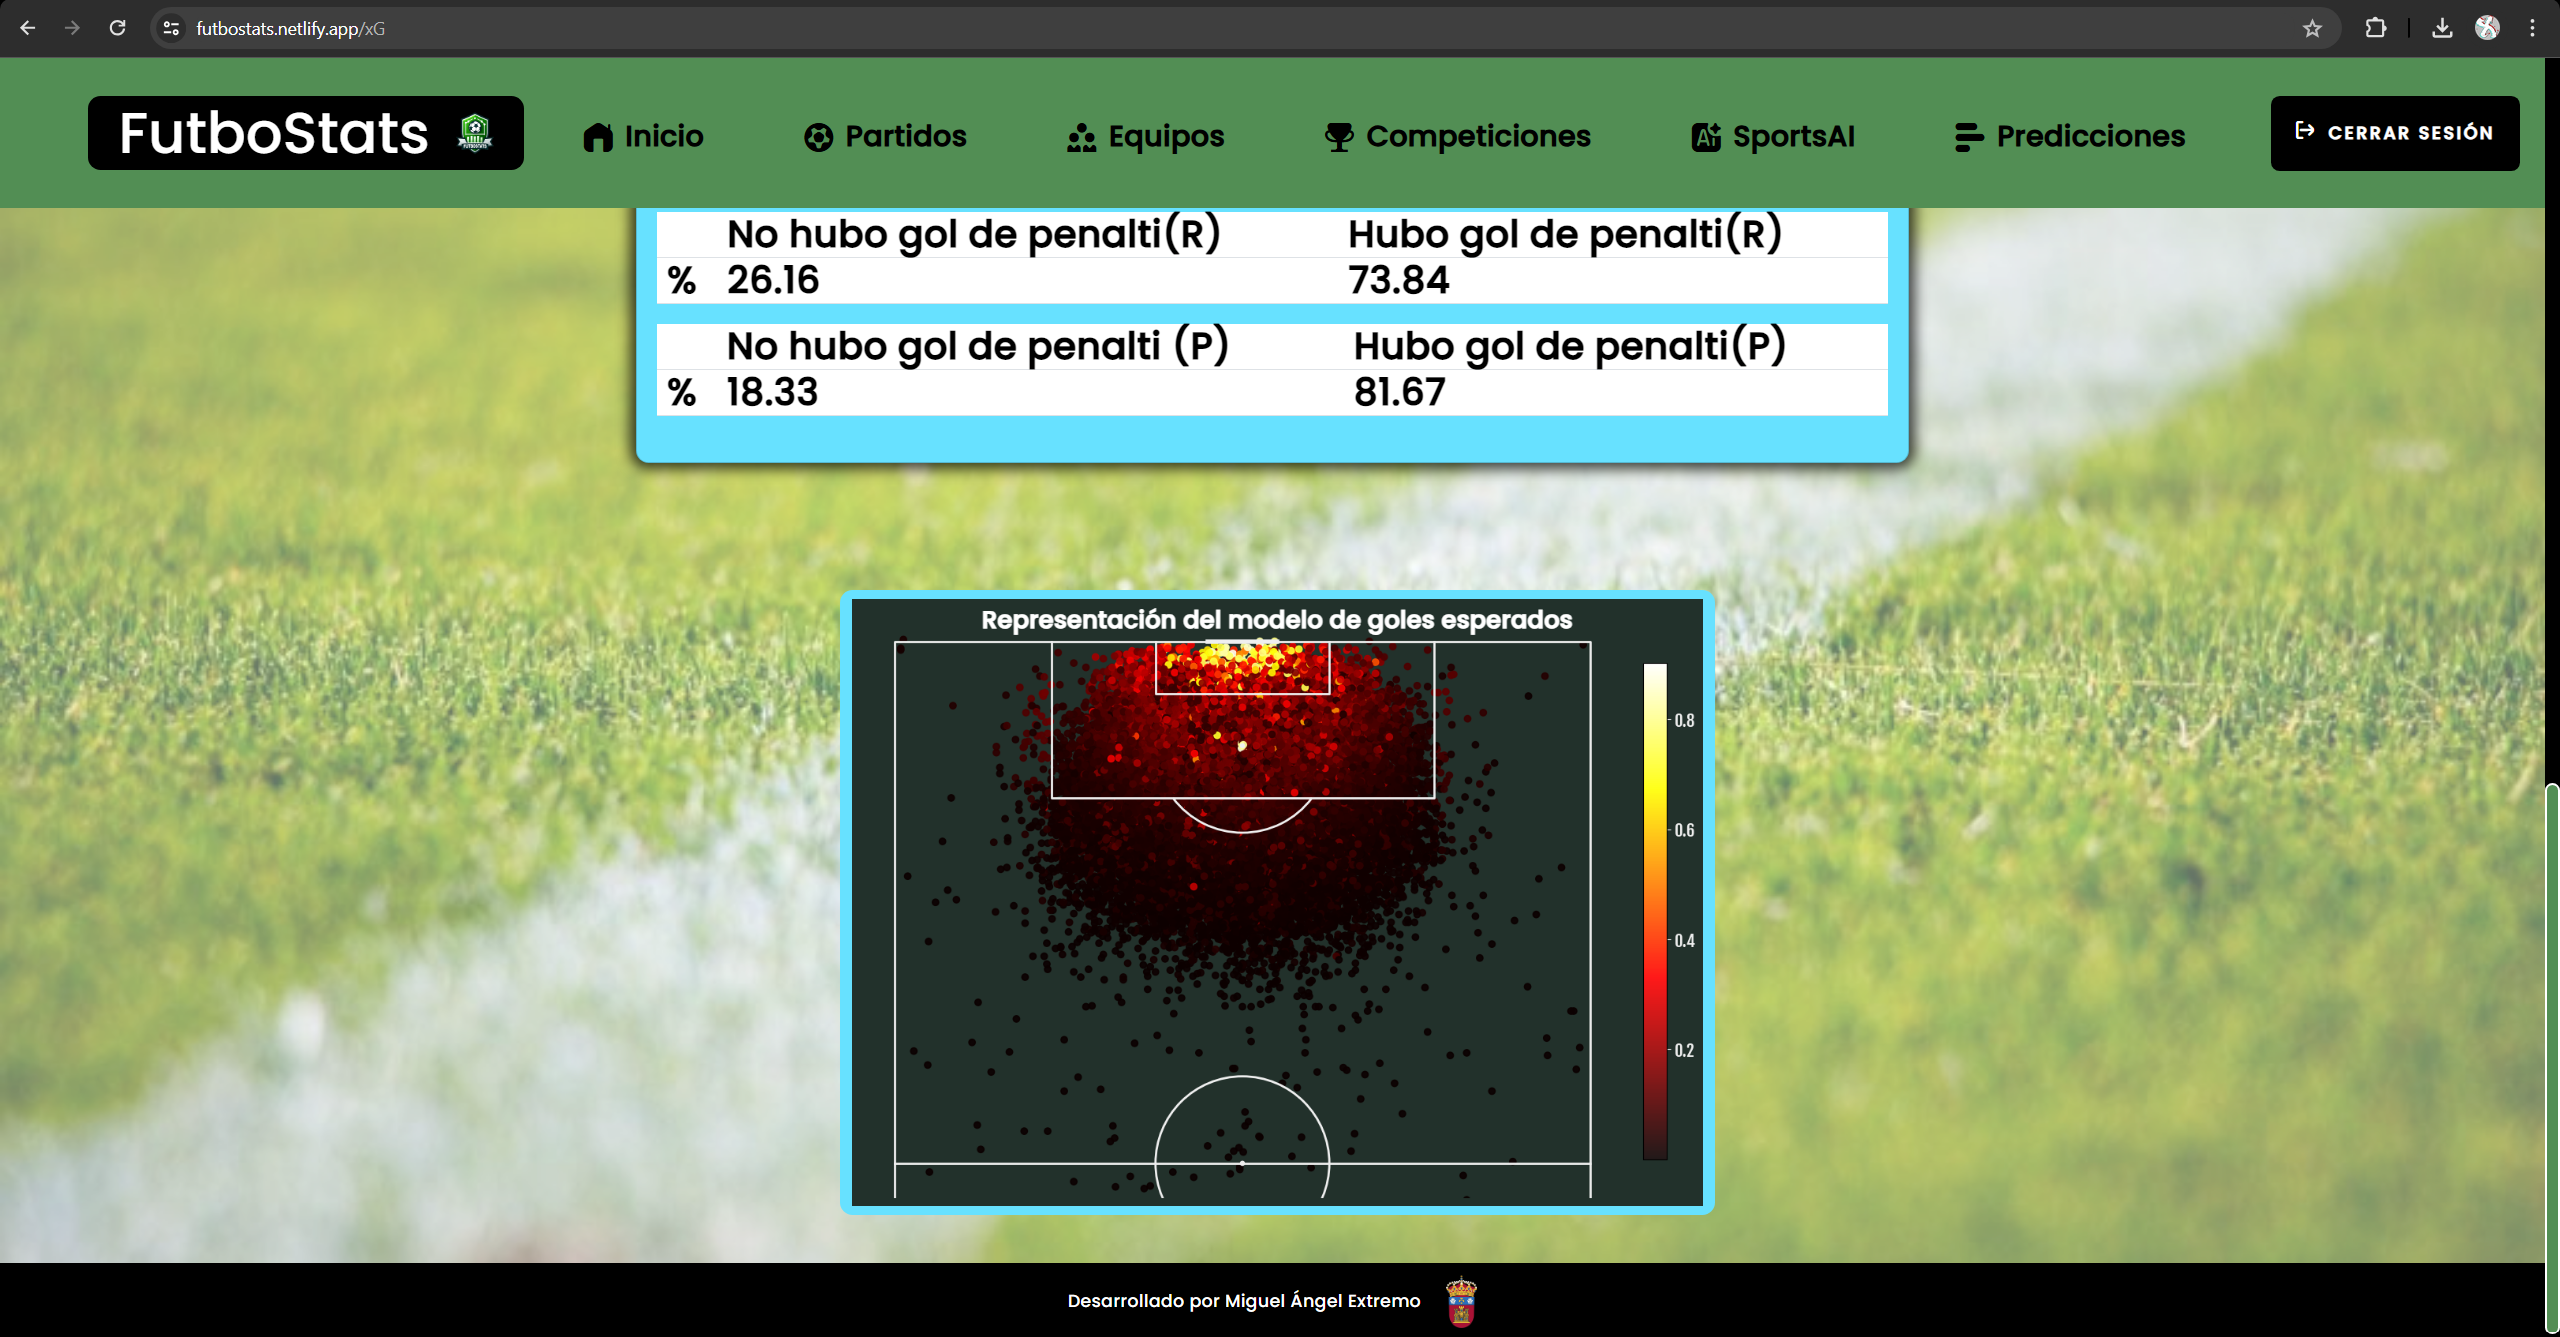
\includegraphics[width=1\linewidth]{img/golesEsperados2-UM.png}
    \caption{Representación gráfica del modelo de goles esperados xG.}
    \label{fig:enter-label}
\end{figure}

\begin{figure}[H]
    \centering
    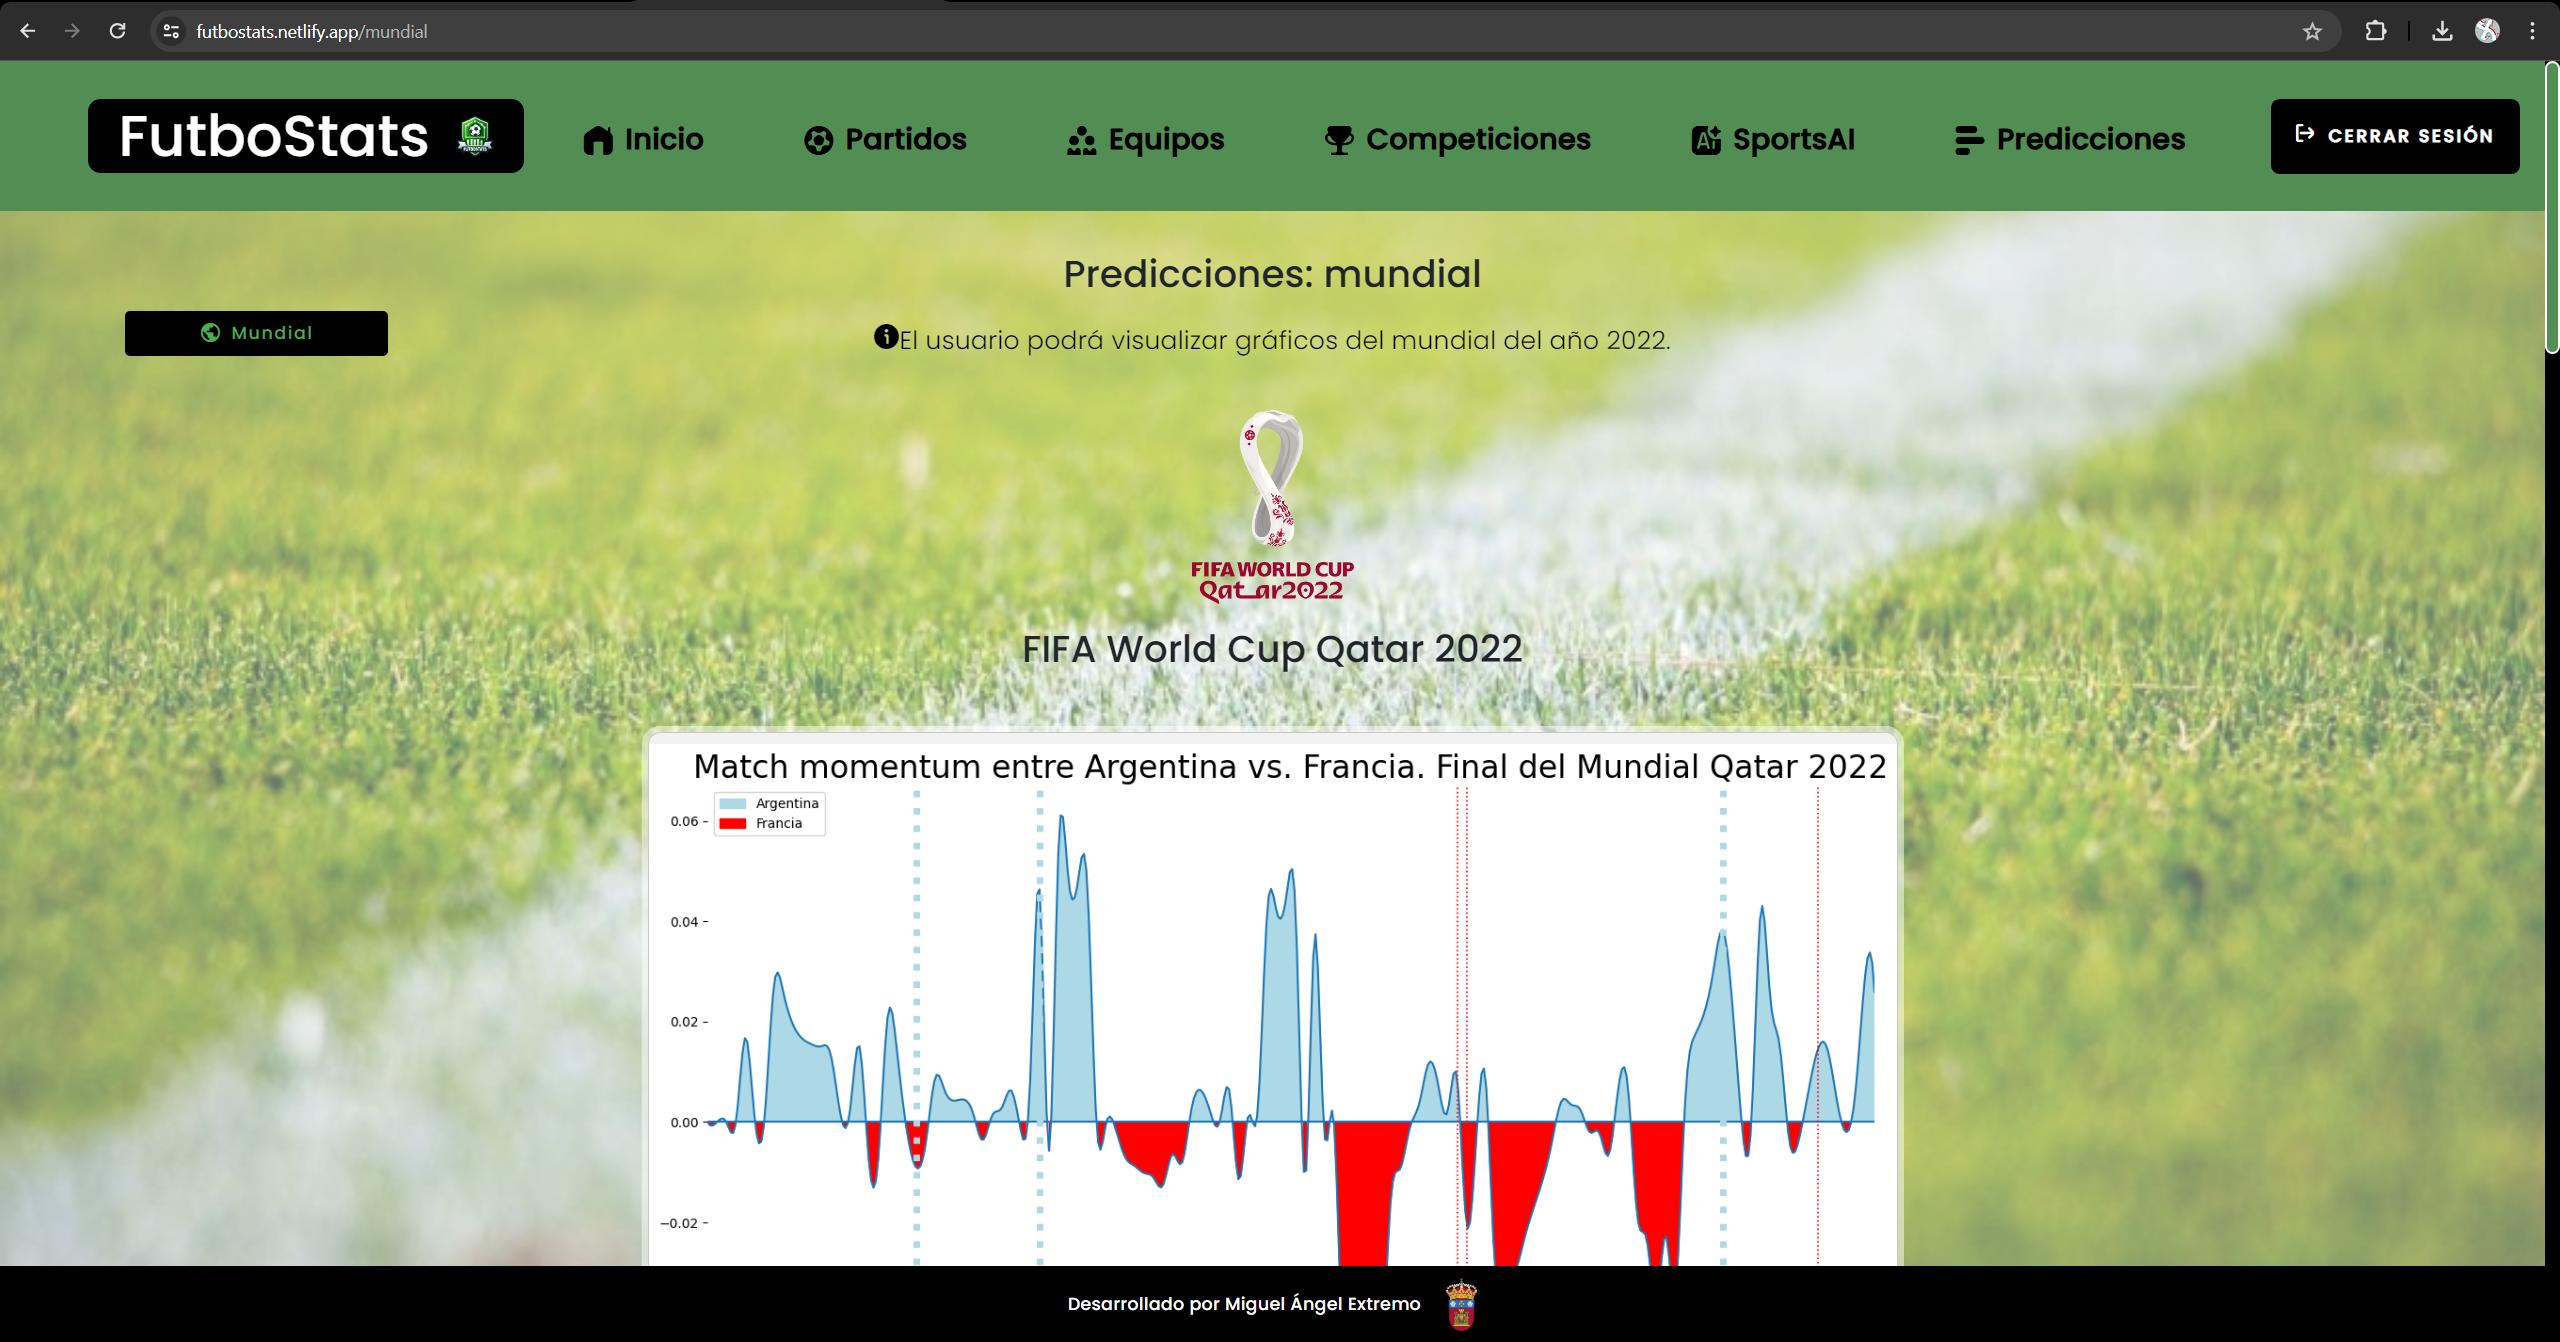
\includegraphics[width=1\linewidth]{img/mundial1-UM.png}
    \caption{Visualización de las estadísticas del mundial 2022}
    \label{fig:enter-label}
\end{figure}

\begin{figure}[H]
    \centering
    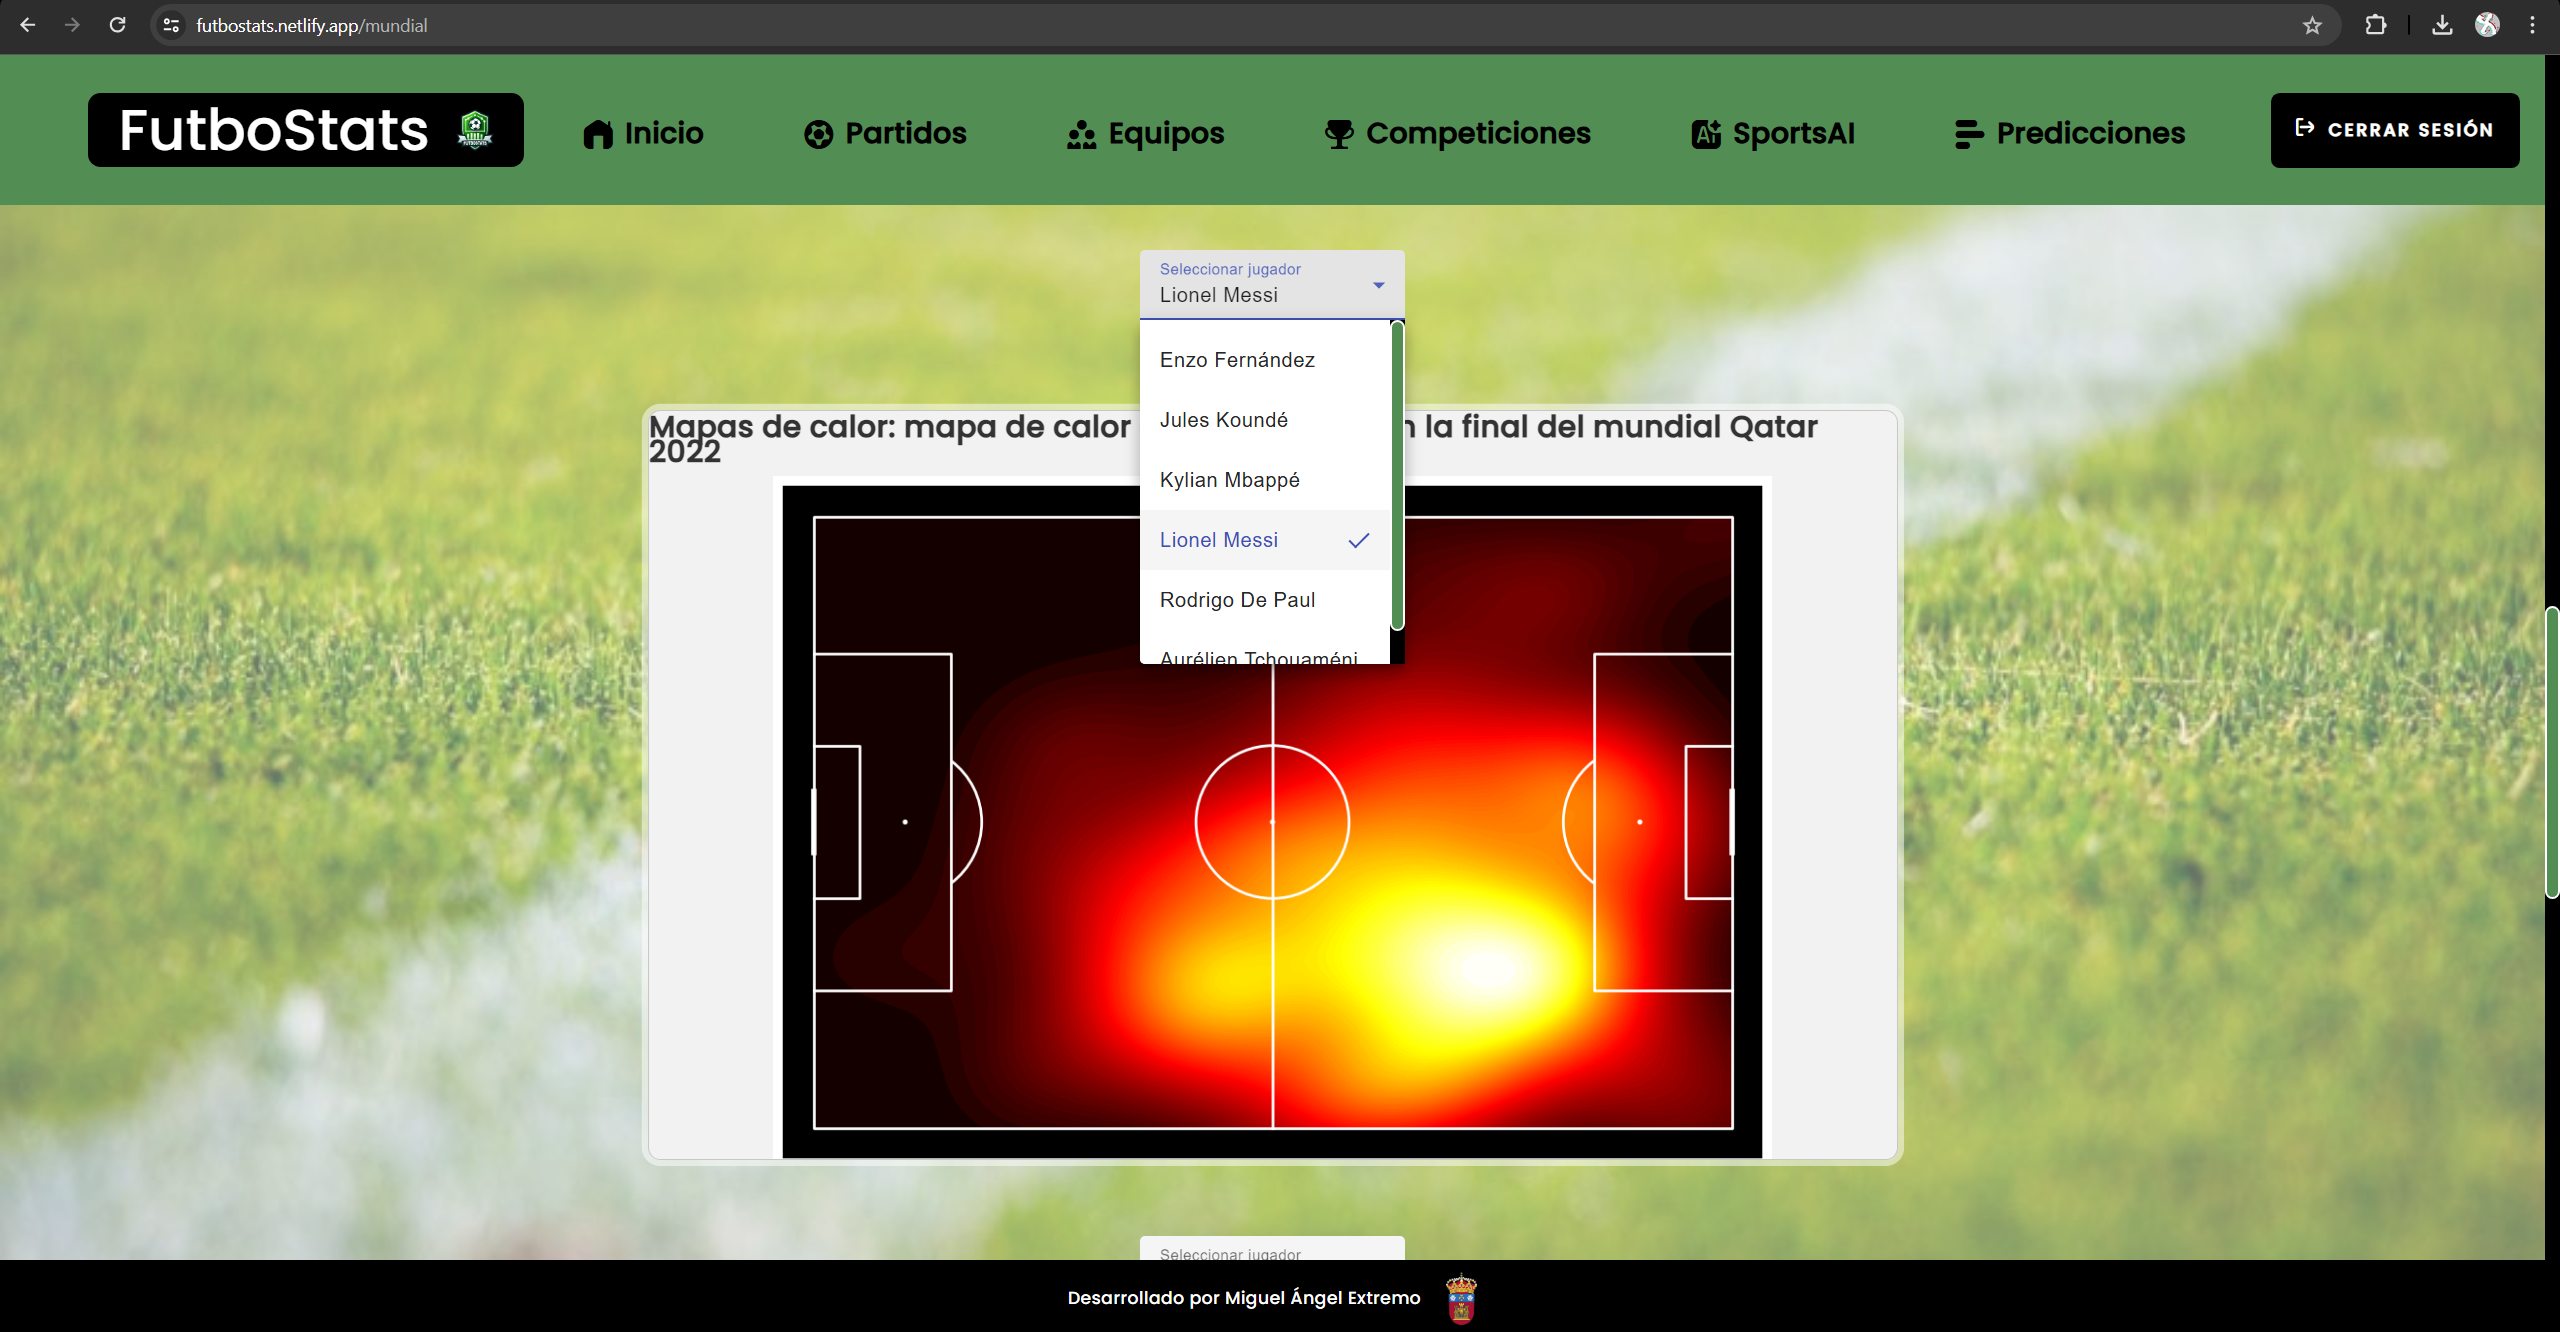
\includegraphics[width=1\linewidth]{img/mundial2-UM.png}
    \caption{Seleccionar el jugador para visualizar su gráfico.}
    \label{fig:enter-label}
\end{figure}

